\documentclass[a4paper,parskip,10pt]{scrartcl}

\usepackage[margin=1.2cm,
%showframe% <- only to show the page layout
paperheight=380mm,
footskip=0.7cm,
]{geometry}

\usepackage[no-math]{fontspec}
%\setmainfont{Montserrat}

\newfontfamily\headingfont[Path=./fonts/]{Montserrat-Medium.ttf}
\newfontfamily\subheadfont[Path=./fonts/]{MontserratAlternates-Regular.ttf}
\newfontfamily\montaltfont[Path=./fonts/]{MontserratAlternates-Regular.ttf}
\newfontfamily\boldfont[Path=./fonts/]{WorkSans-Bold.ttf}
\newfontfamily\mediumfont[Path=./fonts/,BoldFont=WorkSans-Bold.ttf]{WorkSans-Medium.ttf}
\setmainfont[Path=./fonts/,BoldFont=WorkSans-Bold.ttf]{WorkSans-Regular.ttf}

\newfontfamily\timeregularfont[Path=./fonts/]{CooperHewitt-Book.otf}
\newfontfamily\timelightfont[Path=./fonts/]{CooperHewitt-Light.otf}

\usepackage{graphicx}
\usepackage{lipsum}
\usepackage{xcolor}
\usepackage{adjustbox}
\usepackage[most]{tcolorbox}
\usepackage{tikz}
\usepackage{hyperref}
\usepackage{qrcode}
\usepackage{shadowtext}
\usepackage{fontawesome}
\usepackage[style=iso]{datetime2}
\usepackage{scrlayer-scrpage}
\usepackage{lastpage}
\usepackage{xcolor-material}
\usepackage{ragged2e}
\usepackage{microtype}

%\usepackage{newpxmath}
\usepackage{mathspec} 
\setmathfont(Latin,Greek){Gentium Plus}


\usetikzlibrary{fit}

\cfoot{}
\ofoot{\color{white}\footnotesize \thepage/\pageref*{LastPage}}
%\pagestyle{scrheadings}

\AddToHook{shipout/background}{%
    \put (0in,-\paperheight){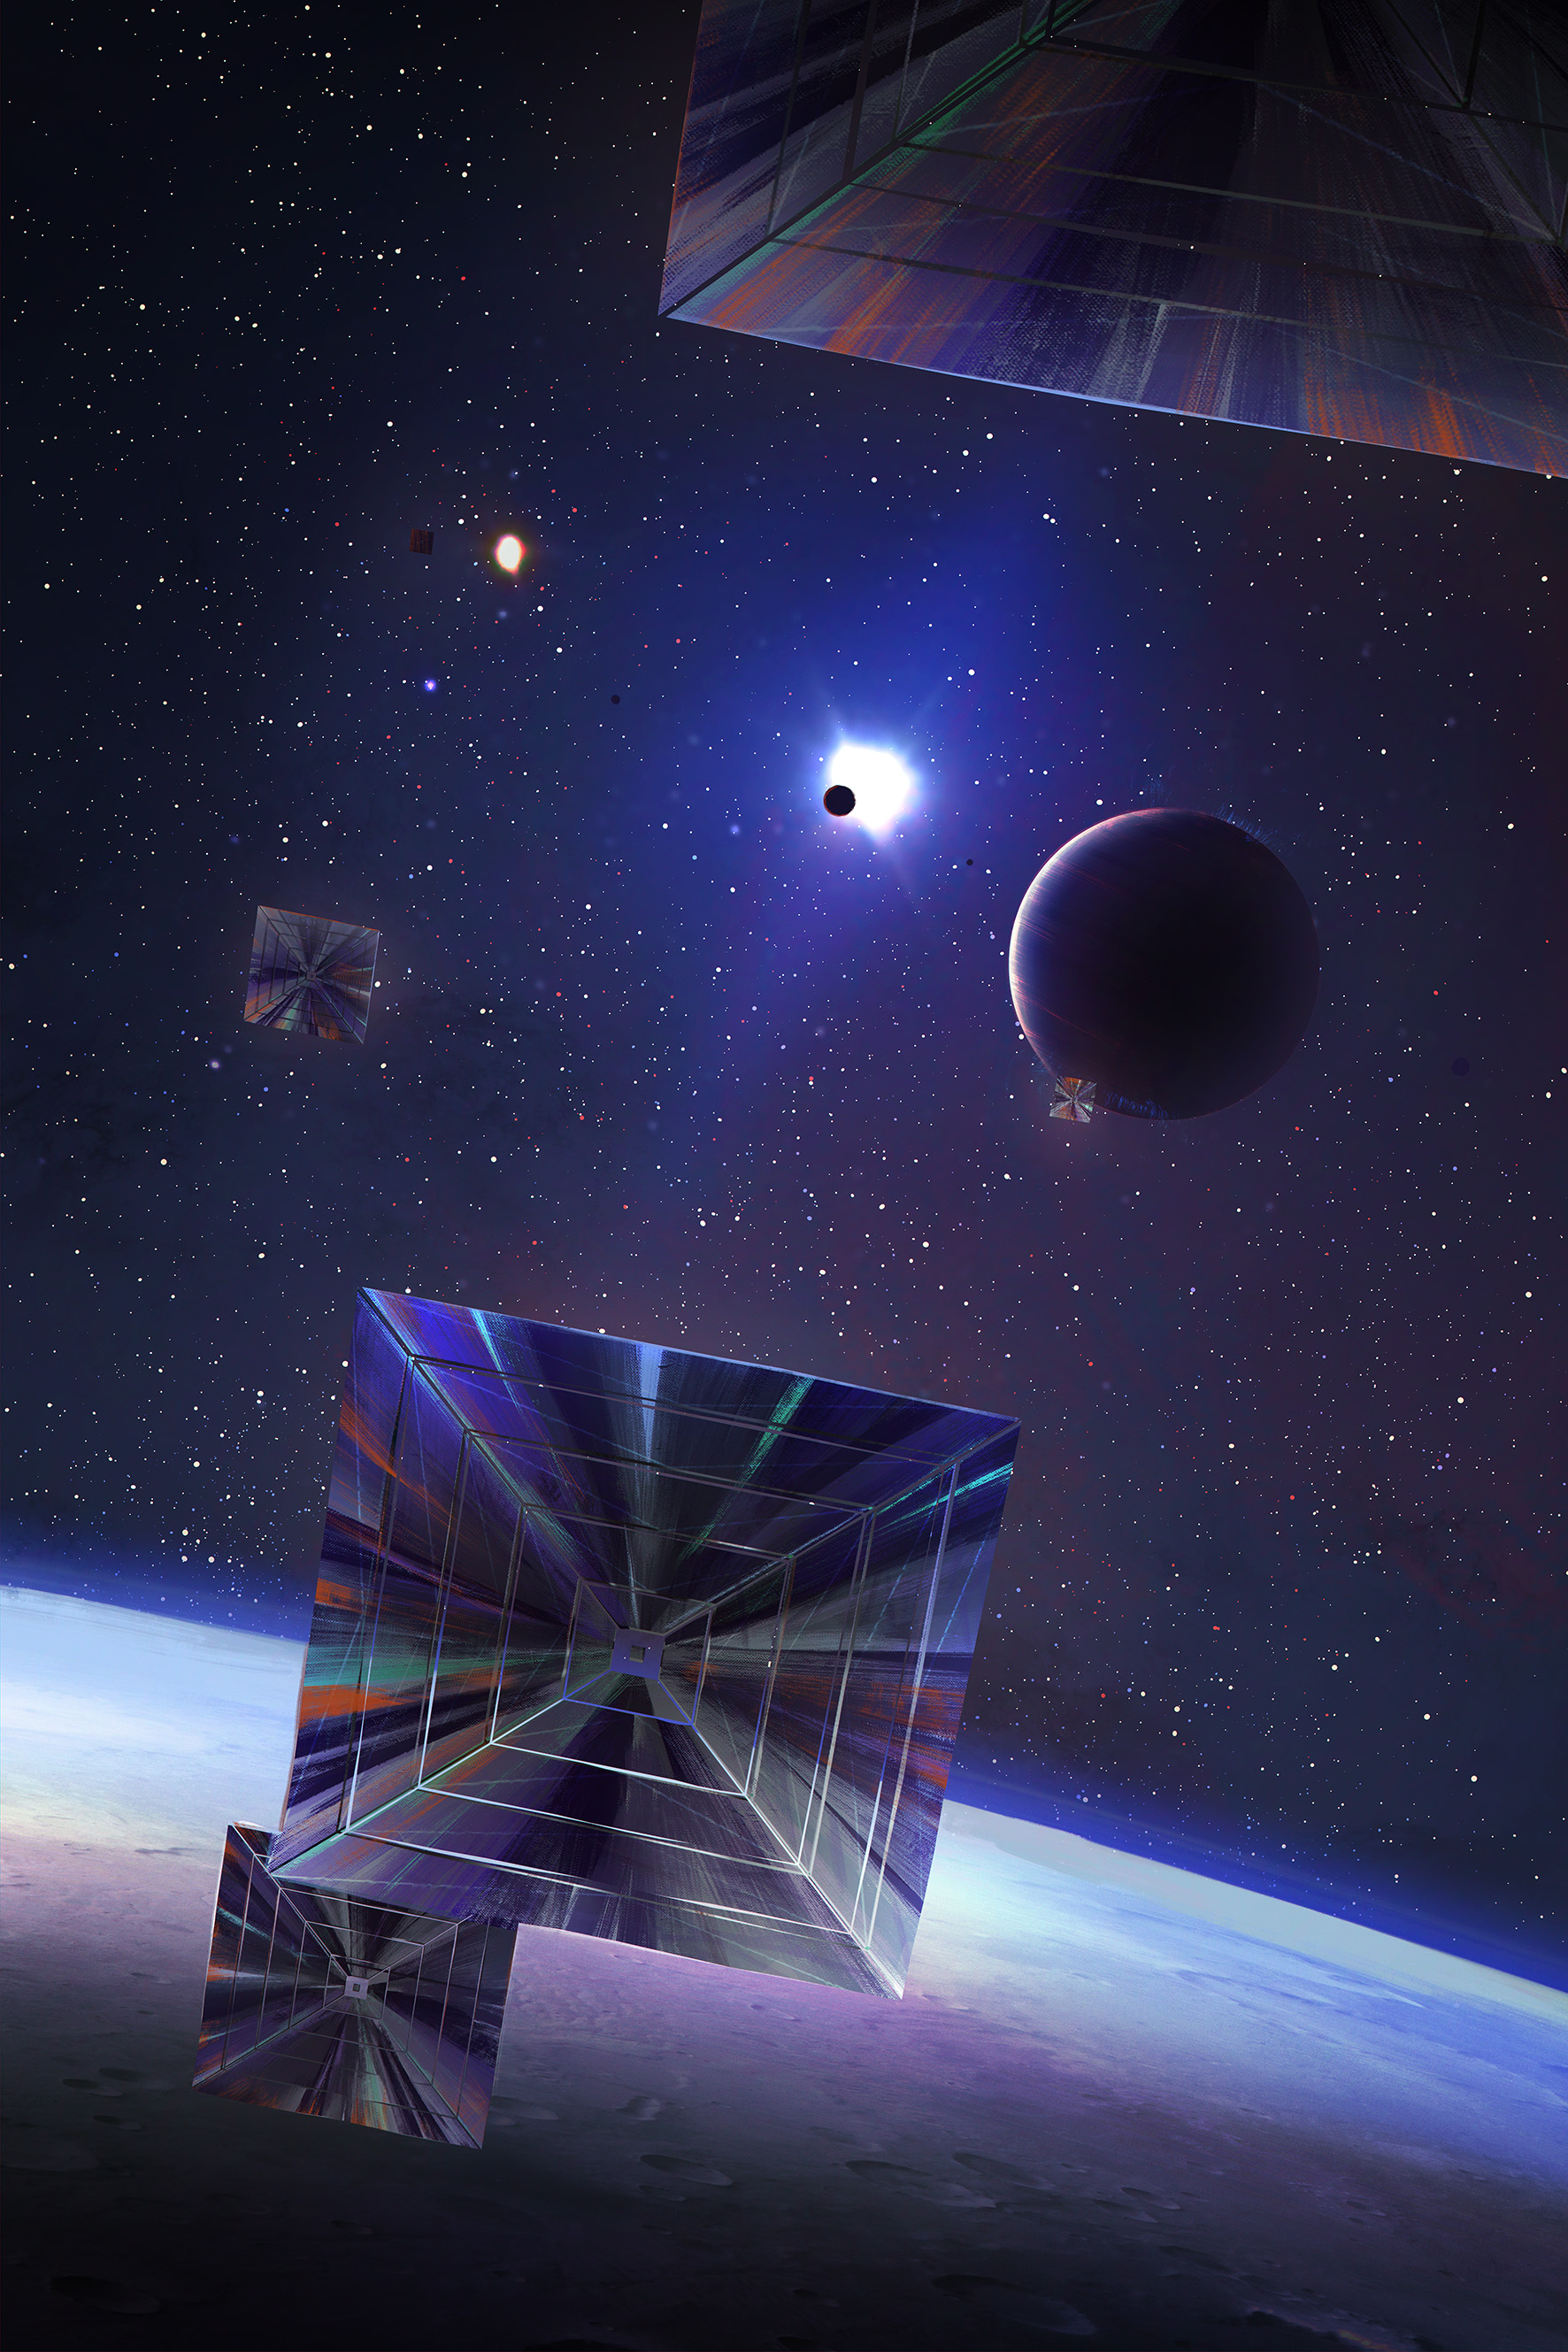
\includegraphics[width=\paperwidth,height=\paperheight]{exoplanetsails_compressed.jpg}}%
}

\definecolor{conference}{HTML}{7F2CA0}

%\AtBeginDocument{
\urlstyle{same}
\hypersetup{%
    colorlinks=false,% hyperlinks will be black
    urlbordercolor=conference,% hyperlink borders will be red
    pdfborderstyle={/S/U/W 1},% border style will be underline of width 1pt
    %
    pdftitle={First European Interstellar Workshop 2024 Schedule},%
    pdfauthor={Konstantinos Kanavouras},%
}
%}

\begin{document}

\begin{centering}
    \color{white}
    \headingfont%
    \Huge First European Interstellar Workshop

    %
\end{centering}

\begin{centering}
    \color{white}
    \subheadfont%
    \LARGE 2\textsuperscript{nd} - 5\textsuperscript{th} December 2024, ECCL, Luxembourg

    %
\end{centering}

    {
        \begin{tikzpicture}
            \node (0,0) {}; % Alignment node for bounding box


            \filldraw[line width=0.7mm,conference] (6,0) rectangle ++(-1.5,1) node[pos=.5,white] {\faExternalLink};
            \draw[line width=0.7mm,draw=conference,fill=black,fill opacity=0.5] (6,0) rectangle ++(6.5,1) node (END) {} node[pos=.5,white,opacity=1] {\large \url{https://feis2024.uni.lu/}};

            \node[fill=white] at (current bounding box.east -| 0,0) {\qrcode[height=2cm]{https://feis2024.uni.lu/schedule?s=qr&qrv=0.24}};
        \end{tikzpicture}%
    }

    \noindent%
    \shadowcolor{black}
    \parbox{.333\textwidth}{\color{white}\footnotesize Version 0.24}%
    \parbox{.333\textwidth}{\color{white}\LARGE \centering \shadowtext{Event Schedule}}%
    \parbox{.333\textwidth}{\hfill\color{white}\footnotesize Updated \today}%





\begin{tcolorbox}[
    width=\paperwidth,
    center,
    boxrule=0pt,
    arc=0pt,
    auto outer arc,
    opacityfill=0.3,
    colframe=black,
    colback=black,
    left=1.2cm,
    right=1.2cm,
    ]
    \color{white}
    {\timeregularfont\fontsize{25}{13.5}\selectfont MONDAY}
    \hspace{.5em}
    \Large \raisebox{.8ex}{%
    December %
    2%
    %
    nd%
    %
    %
    }
    \hfill
    \raisebox{.8ex}{
    \begin{tikzpicture}
        \def\spacing{0.3}
        \def\size{0.3}
        %\fill[fill=conference!30!black] (0,0) rectangle ++(0.2,0.2);
        %\fill[fill=conference!90!black] (0.4,0) rectangle ++(0.2,0.2);
        %\fill[fill=conference!30!black] (0.8,0) rectangle ++(0.2,0.2);
        %\fill[fill=conference!30!black] (1.2,0) rectangle ++(0.2,0.2);
        \foreach \i in {0,1,2,3} {
            \def\basecolor{conference}
            \def\color{\basecolor!30!gray!50!black}
            \ifnum \i = 0
                \def\color{\basecolor!90!white}
            \fi
            \fill[fill=\color] ({\i*(\spacing+\size)},0) rectangle ++(\size,\size);
        }
    \end{tikzpicture}
    }
\end{tcolorbox}



\begin{tcolorbox}[width=\linewidth,center,boxrule=0pt,arc=0pt,auto outer arc,colframe=white,breakable,height fixed for=all]
    
    \begin{tikzpicture}

        \node at (-1,0) {}; % Alignment node for bounding box

        

            \fill[rounded corners=1mm,gray!50!white]
            (1,-0.7) rectangle (16.2,0.7) node[pos=.5,gray!50!black] {\mediumfont Registration opens};

            \node[anchor=south] (S) at (current bounding box.west -| 0,0) {\timeregularfont\Large 08:45 };
            \node[anchor=north] (E) at (current bounding box.west -| 0,0) {\timelightfont\textendash~ 09:00 };     

        

   

        % bottom padding
        \path (current bounding box.south) ++(0,-1mm) node[anchor=north] {};
    \end{tikzpicture}
    %\vspace{0mm plus 3cm}
    \vspace{0cm plus 1cm minus 2mm}
    %\vfill
    
    \begin{tikzpicture}

        \node at (-1,0) {}; % Alignment node for bounding box

        
            \definecolor{thistrack}{HTML}{7f2ca0}

            \def\x{1.3}
            \def\width{14cm}

            

            \node[anchor=west,text width=\width,align=left,minimum height=1.3cm] (T) at (\x,0) {\mediumfont%
            Introductory Seminars%
            %
            %
                %~\\[1ex]%
                {%
                \par%
                \justifying%
                \setlength{\parskip}{1ex}
                %\color{thistrack!20!black}%
                \small%
                \fontfamily{\familydefault}\selectfont%
                Seminars are 3-hour presentations on a single subject presented by individuals familiar with the topic and providing an in-depth look at that subject. Seminars are not included in the IRG Symposium costs and do not require Symposium membership to attend.

The seminar topics are: \begin{itemize}
  \item Interstellar Generation Ships \textemdash~Designing Miniaturized Worlds (Andreas M.~Hein)
  \item Planning for the Truly Long Long-Term (Anders Sandberg)
  \item Interstellar Propulsion: Current Prospects and Future Possibilities (Les Johnson)
\end{itemize}

The seminar venue will be the University of Luxembourg.

For registration and more information, please visit: {\color{conference!50!black}\url{https://feis2024.uni.lu/seminars}}
%
                }%
            %
            %
                %%
            %
            %
            };

            
            % Draw rounded rectangle next to that
            
            \fill[rounded corners=1mm,thistrack] (T.north west -| 1,-1) rectangle (T.south west -| 1.2,1) {};
            

            \node[anchor=south] (S) at (current bounding box.west -| 0,0) {\timeregularfont\Large 09:00 };
            \node[anchor=north] (E) at (current bounding box.west -| 0,0) {\timelightfont\textendash~ 16:00 };    
            
            
                \node[anchor=north east,rounded corners=1mm,fill=thistrack,inner sep=2mm,text width=1.7cm,align=center,xshift=1.7mm,yshift=0.1mm] 
                    at (T.north west -| 1,-1) {\color{white}\small SIGN UP REQUIRED};
            

            %

        

   

        % bottom padding
        \path (current bounding box.south) ++(0,-1mm) node[anchor=north] {};
    \end{tikzpicture}
    %\vspace{0mm plus 3cm}
    \vspace{0cm plus 1cm minus 2mm}
    %\vfill
    
    \begin{tikzpicture}

        \node at (-1,0) {}; % Alignment node for bounding box

        
            \definecolor{thistrack}{HTML}{7f2ca0}

            \def\x{1.3}
            \def\width{14cm}

            

            \node[anchor=west,text width=\width,align=left,minimum height=1.3cm] (T) at (\x,0) {\mediumfont%
            Opening Reception%
            %
            %
            %
                %%
            %
            %
                \\[0ex]%
                \color{gray}\footnotesize%
                ECCL, La Table du Belvédère%%
            };

            
            % Draw rounded rectangle next to that
            
            \fill[rounded corners=1mm,thistrack] (T.north west -| 1,-1) rectangle (T.south west -| 1.2,1) {};
            

            \node[anchor=south] (S) at (current bounding box.west -| 0,0) {\timeregularfont\Large 16:30 };
            \node[anchor=north] (E) at (current bounding box.west -| 0,0) {\timelightfont\textendash~ 18:00 };    
            
            

            %

        

   

        % bottom padding
        \path (current bounding box.south) ++(0,-1mm) node[anchor=north] {};
    \end{tikzpicture}
    %\vspace{0mm plus 3cm}
    \vspace{0cm plus 1cm minus 2mm}
    %\vfill
    
    \begin{tikzpicture}

        \node at (-1,0) {}; % Alignment node for bounding box

        
            \definecolor{thistrack}{HTML}{5FAB5D}

            \def\x{1.3}
            \def\width{14cm}

            

            \node[anchor=west,text width=\width,align=left,minimum height=1.3cm] (T) at (\x,0) {\mediumfont%
            Science Fiction Authors Night%
            %
            %
                %~\\[1ex]%
                {%
                \par%
                \justifying%
                \setlength{\parskip}{1ex}
                %\color{thistrack!20!black}%
                \small%
                \fontfamily{\familydefault}\selectfont%
                The first public event of the FEIS2024 symposium will feature three prominent Science Fiction authors, and will be open to all space professionals and enthusiasts on December 2\textsuperscript{nd}.

    \begin{tcolorbox}[
      frame hidden,
      sidebyside,
      bicolor,
      colback=thistrack!70!black,
      colbacklower=thistrack!90!black,
      size=title,
      top=1mm,
      bottom=1mm,
      boxrule=0pt,
      lefthand ratio=0.5,
      sidebyside align=center,
      halign=center,
      halign lower=flush center,
      % title={  },
  ]%
      \color{white}%
      \textbf{%
          FREE REGISTRATION REQUIRED%%
      }%
      \tcblower%
      \color{white}%
      \url{https://feis2024.uni.lu/register/authors}%
  \end{tcolorbox}


\begin{minipage}[c]{0.2\linewidth}
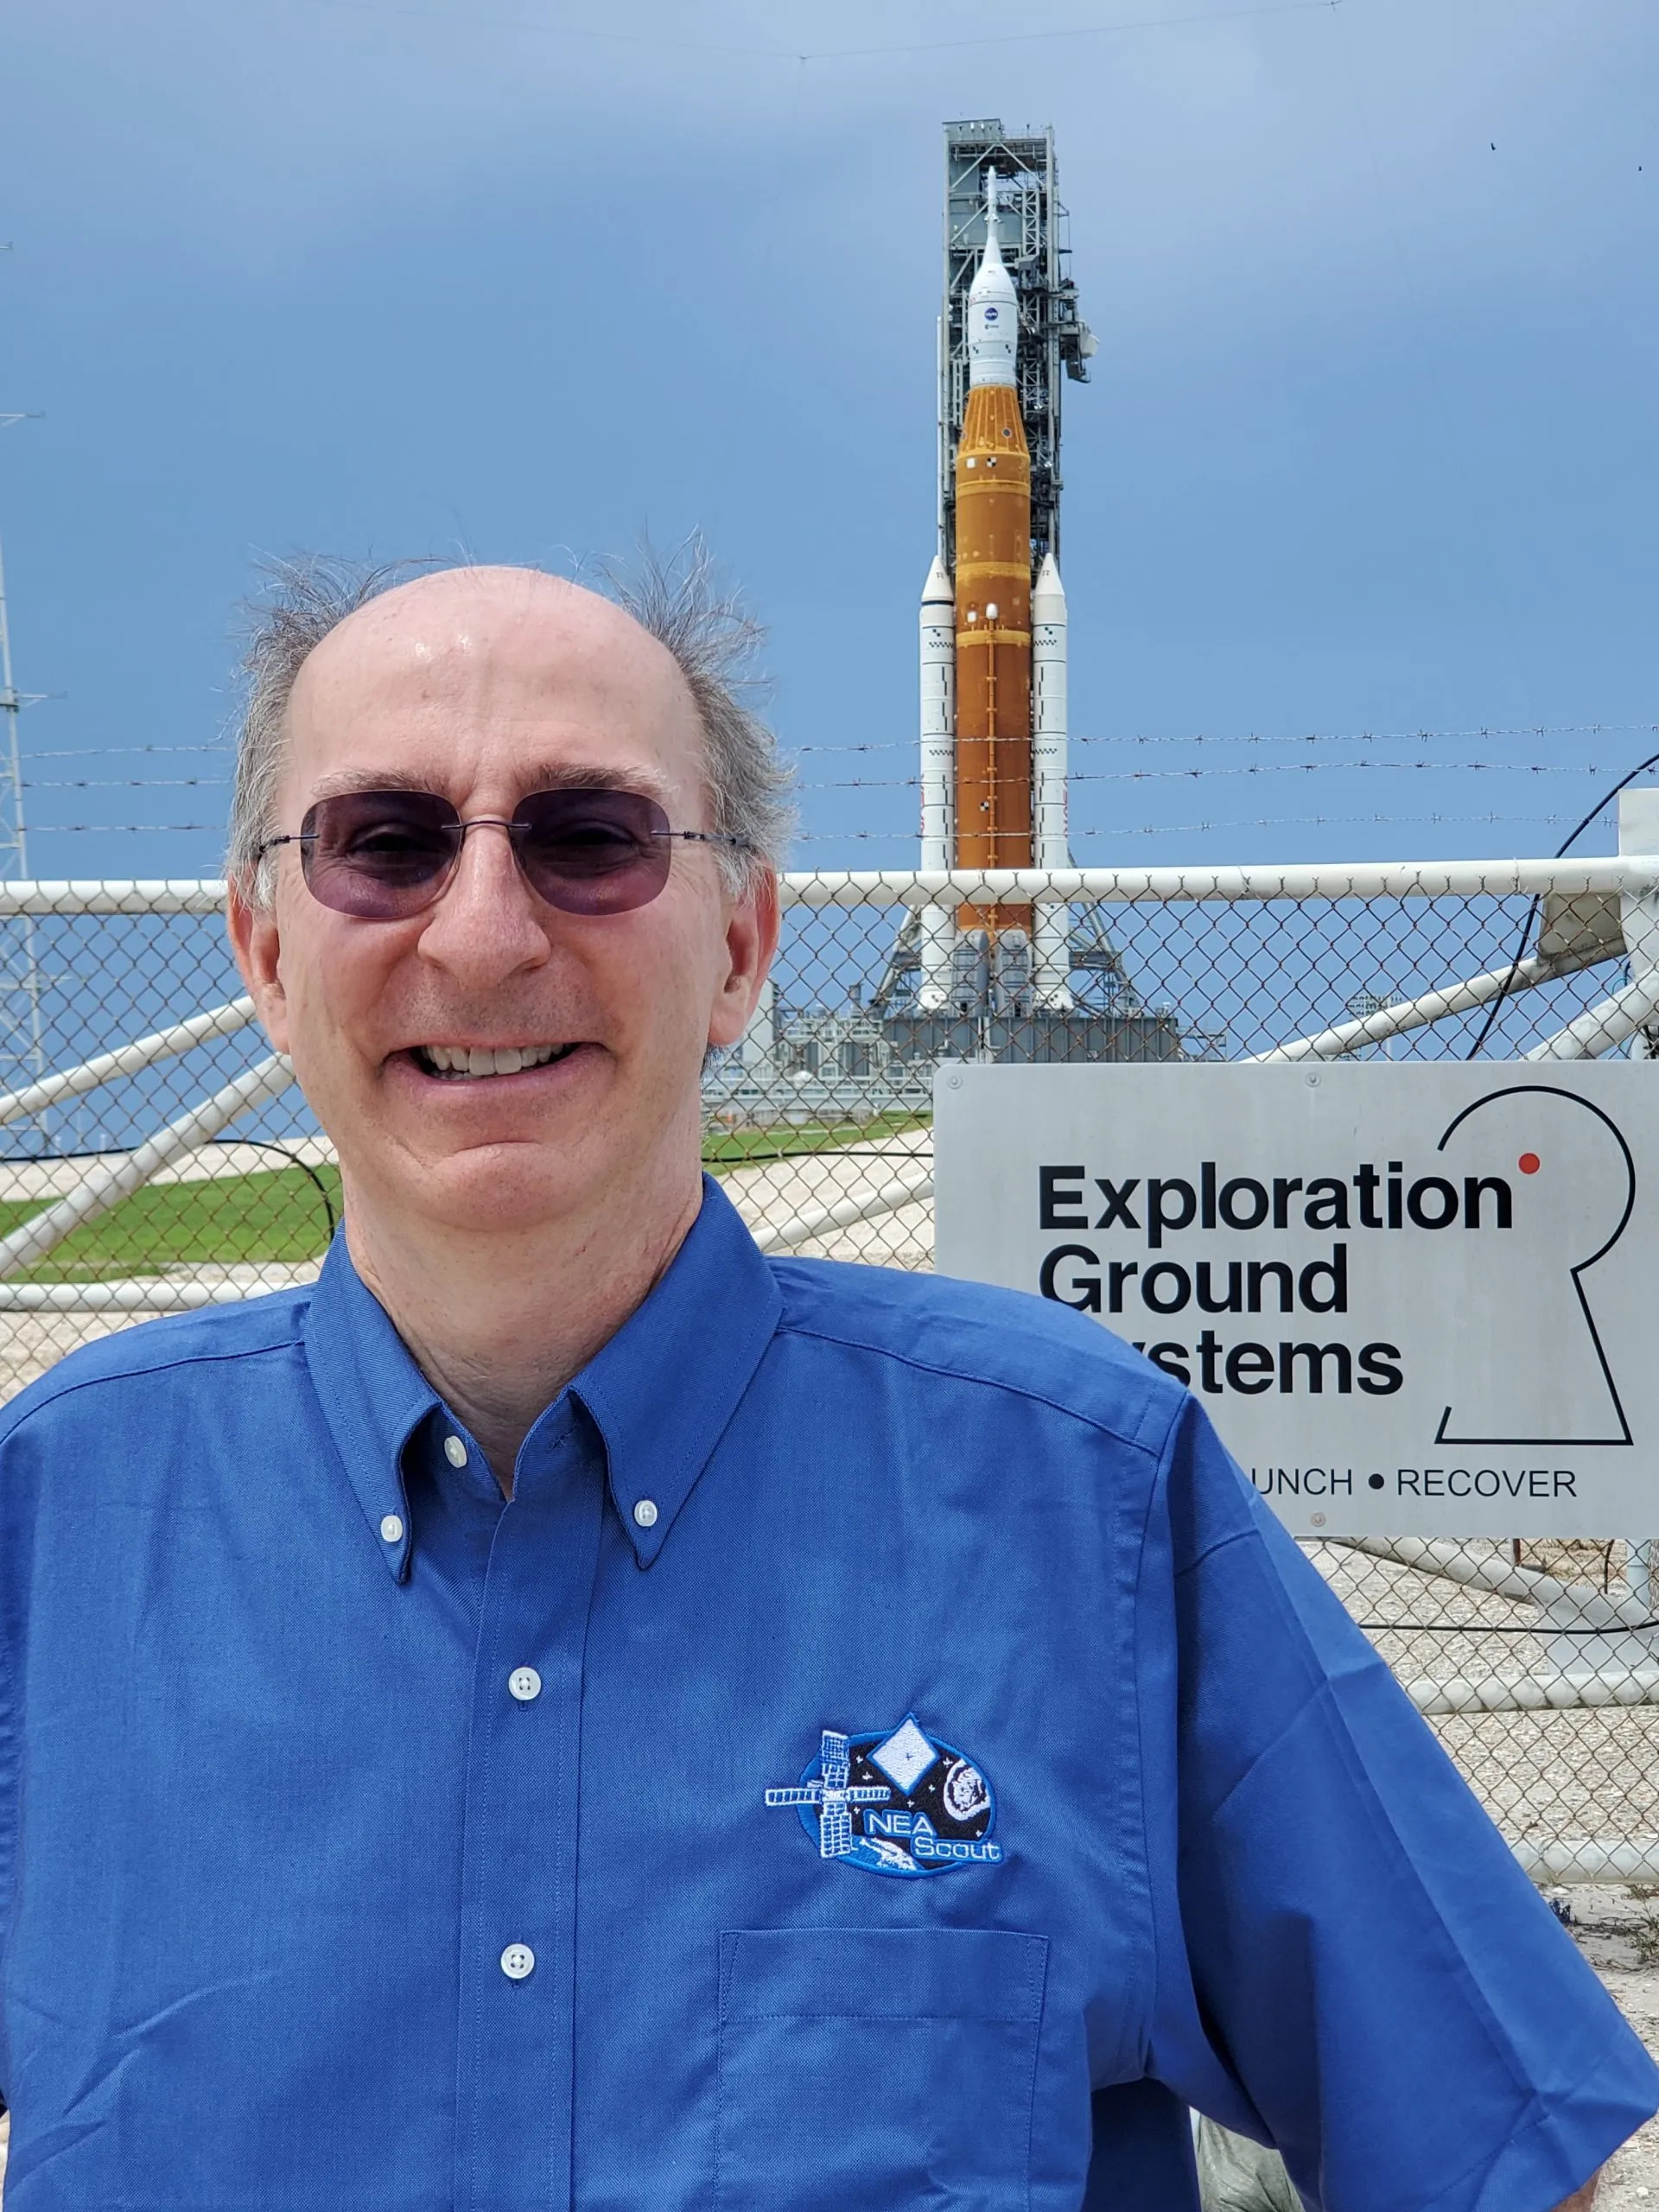
\includegraphics[width=\textwidth]{media/author1.jpg}
\end{minipage}~
\begin{minipage}[c]{0.8\linewidth}
\textbf{Les Johnson} is a physicist, award-winning science and science fiction author, and Chief Technologist at the NASA George C.~Marshall Space Flight Center.
%His science fiction books include Crisis at Proxima (Baen 2024), The Ross 248 Project (Baen 2023), Saving Proxima (Baen 2021), Pluto: The Dark World (coming from Tor 2025), and more. Les's popular science books include A Traveler's Guide to the Stars (Princeton Press 2022) \textemdash~now translated into 7 languages, Graphene: The Superstrong, Superthin, and Superversatile Material That Will Revolutionize the World (2018), Solar Sails: A Novel Approach to Interplanetary Travel, and others.
He was a technical consultant for the movies Europa Report, Lost in Space, and Solis. NPR, CNN, Fox News, The Science Channel and The Discovery Channel have all interviewed Les about space and space exploration. Les was the featured Interstellar Explorer in the January 2013 issue of National Geographic magazine and appeared there again in March 2019.
\end{minipage}

\begin{minipage}[c]{0.2\linewidth}
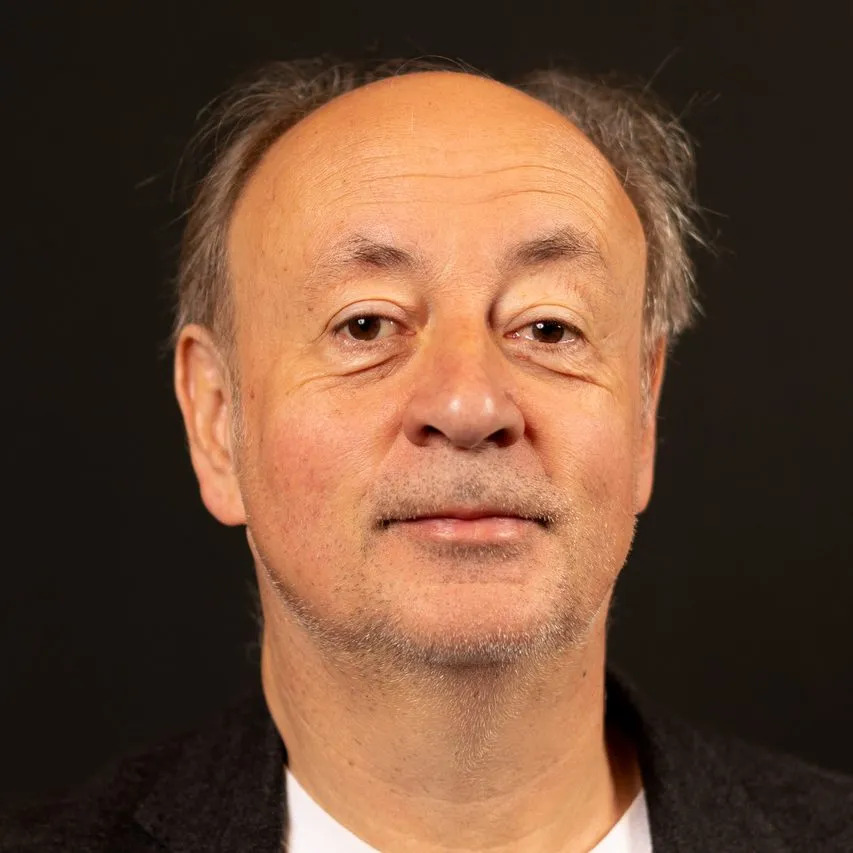
\includegraphics[width=\textwidth]{media/author2.jpg}
\end{minipage}~
\begin{minipage}[c]{0.8\linewidth}
\textbf{Brandon Q. Morris} is a physicist and space specialist. He has long been concerned with space issues, both professionally and privately and while he wanted to become an astronaut, he had to stay on Earth for a variety of reasons. He is particularly fascinated by the “what if” and through his books he aims to share compelling hard science fiction stories that could actually happen, and someday may happen.
\end{minipage}

\begin{minipage}[c]{0.2\linewidth}

\includegraphics[width=\textwidth]{media/author3.jpg}
\end{minipage}~
\begin{minipage}[c]{0.8\linewidth}
With almost 2 million books sold, \textbf{Joshua T. Calvert} is at the forefront of current international science fiction. His German novel “Singularity”, published by Fischer-Tor, won the prestigious “Seraph” fantasy literature prize for best novel in 2022. The English translation of his Kindle hit “The Fossil” won second place in the 2021 American “Reader’s Favorite Awards” for best novel. His books are available in English, Spanish and German. % As a hybrid author, his novels are indie-published and published by well-known publishers.
He lives with his wife and son between Portugal and Greece. 
\end{minipage}
%
                }%
            %
            %
                %%
            %
            %
            };

            
            % Draw rounded rectangle next to that
            
            \fill[rounded corners=1mm,thistrack] (T.north west -| 1,-1) rectangle (T.south west -| 1.2,1) {};
            

            \node[anchor=south] (S) at (current bounding box.west -| 0,0) {\timeregularfont\Large 18:30 };
            \node[anchor=north] (E) at (current bounding box.west -| 0,0) {\timelightfont\textendash~ 19:45 };    
            
            
                \node[anchor=north east,rounded corners=1mm,fill=thistrack,inner sep=2mm,text width=1.7cm,align=center,xshift=1.7mm,yshift=0.1mm] 
                    at (T.north west -| 1,-1) {\color{white}\small OPEN TO PUBLIC};
            

            %

        

   

        % bottom padding
        \path (current bounding box.south) ++(0,-1mm) node[anchor=north] {};
    \end{tikzpicture}
    %\vspace{0mm plus 3cm}
    \vspace{0cm plus 1cm minus 2mm}
    %\vfill
    
    \begin{tikzpicture}

        \node at (-1,0) {}; % Alignment node for bounding box

        

            \fill[rounded corners=1mm,gray!50!white]
            (1,-0.7) rectangle (16.2,0.7) node[pos=.5,gray!50!black] {\mediumfont Space Cafe};

            \node[anchor=south] (S) at (current bounding box.west -| 0,0) {\timeregularfont\Large 19:45 };
            \node[anchor=north] (E) at (current bounding box.west -| 0,0) {\timelightfont\textendash~ 21:30 };     

        

   

        % bottom padding
        \path (current bounding box.south) ++(0,-1mm) node[anchor=north] {};
    \end{tikzpicture}
    %\vspace{0mm plus 3cm}
    \vspace{0cm plus 1cm minus 2mm}
    %\vfill
    

\end{tcolorbox}




\newpage


\begin{tcolorbox}[
    width=\paperwidth,
    center,
    boxrule=0pt,
    arc=0pt,
    auto outer arc,
    opacityfill=0.3,
    colframe=black,
    colback=black,
    left=1.2cm,
    right=1.2cm,
    ]
    \color{white}
    {\timeregularfont\fontsize{25}{13.5}\selectfont TUESDAY}
    \hspace{.5em}
    \Large \raisebox{.8ex}{%
    December %
    3%
    %
    %
    rd%
    %
    }
    \hfill
    \raisebox{.8ex}{
    \begin{tikzpicture}
        \def\spacing{0.3}
        \def\size{0.3}
        %\fill[fill=conference!30!black] (0,0) rectangle ++(0.2,0.2);
        %\fill[fill=conference!90!black] (0.4,0) rectangle ++(0.2,0.2);
        %\fill[fill=conference!30!black] (0.8,0) rectangle ++(0.2,0.2);
        %\fill[fill=conference!30!black] (1.2,0) rectangle ++(0.2,0.2);
        \foreach \i in {0,1,2,3} {
            \def\basecolor{conference}
            \def\color{\basecolor!30!gray!50!black}
            \ifnum \i = 1
                \def\color{\basecolor!90!white}
            \fi
            \fill[fill=\color] ({\i*(\spacing+\size)},0) rectangle ++(\size,\size);
        }
    \end{tikzpicture}
    }
\end{tcolorbox}



\begin{tcolorbox}[width=\linewidth,center,boxrule=0pt,arc=0pt,auto outer arc,colframe=white,breakable,height fixed for=all]
    
    \begin{tikzpicture}

        \node at (-1,0) {}; % Alignment node for bounding box

        

            \fill[rounded corners=1mm,gray!50!white]
            (1,-0.7) rectangle (16.2,0.7) node[pos=.5,gray!50!black] {\mediumfont Registration};

            \node[anchor=south] (S) at (current bounding box.west -| 0,0) {\timeregularfont\Large 08:10 };
            \node[anchor=north] (E) at (current bounding box.west -| 0,0) {\timelightfont\textendash~ 08:40 };     

        

   

        % bottom padding
        \path (current bounding box.south) ++(0,-1mm) node[anchor=north] {};
    \end{tikzpicture}
    %\vspace{0mm plus 3cm}
    \vspace{0cm plus 1cm minus 2mm}
    %\vfill
    
    \begin{tikzpicture}

        \node at (-1,0) {}; % Alignment node for bounding box

        
            \definecolor{thistrack}{HTML}{7f2ca0}

            \def\x{1.3}
            \def\width{14cm}

            

            \node[anchor=west,text width=\width,align=left,minimum height=1.3cm] (T) at (\x,0) {\mediumfont%
            Welcome by the organizers, Conference Agenda Review%
            %
            %
            %
                %%
            %
            %
            };

            
            % Draw rounded rectangle next to that
            
            \fill[rounded corners=1mm,thistrack] (T.north west -| 1,-1) rectangle (T.south west -| 1.2,1) {};
            

            \node[anchor=south] (S) at (current bounding box.west -| 0,0) {\timeregularfont\Large 08:40 };
            \node[anchor=north] (E) at (current bounding box.west -| 0,0) {\timelightfont\textendash~ 09:00 };    
            
            

            %

        

   

        % bottom padding
        \path (current bounding box.south) ++(0,-1mm) node[anchor=north] {};
    \end{tikzpicture}
    %\vspace{0mm plus 3cm}
    \vspace{0cm plus 1cm minus 2mm}
    %\vfill
    
    \begin{tikzpicture}

        \node at (-1,0) {}; % Alignment node for bounding box

        
            \definecolor{thistrack}{HTML}{202020}

            \def\x{1.3}
            \def\width{14cm}

            

            \node[anchor=west,text width=\width,align=left,minimum height=1.3cm] (T) at (\x,0) {\mediumfont%
            \textbf{Keynote:}\ %
            Pete Worden (Breakthrough Initiatives): Life in the Universe and Private Sector Space Science Initiatives%
            %
            %
            %
            %
            };

            
            % Draw rounded rectangle next to that
            
            \fill[rounded corners=1mm,thistrack] (T.north west -| 1,-1) rectangle (T.south west -| 1.2,1) {};
            

            \node[anchor=south] (S) at (current bounding box.west -| 0,0) {\timeregularfont\Large 09:00 };
            \node[anchor=north] (E) at (current bounding box.west -| 0,0) {\timelightfont\textendash~ 09:50 };    
            
            

            %

        

   

        % bottom padding
        \path (current bounding box.south) ++(0,-1mm) node[anchor=north] {};
    \end{tikzpicture}
    %\vspace{0mm plus 3cm}
    \vspace{0cm plus 1cm minus 2mm}
    %\vfill
    
    \begin{tikzpicture}

        \node at (-1,0) {}; % Alignment node for bounding box

        

            \fill[rounded corners=1mm,gray!50!white]
            (1,-0.7) rectangle (16.2,0.7) node[pos=.5,gray!50!black] {\mediumfont Coffee break};

            \node[anchor=south] (S) at (current bounding box.west -| 0,0) {\timeregularfont\Large 09:50 };
            \node[anchor=north] (E) at (current bounding box.west -| 0,0) {\timelightfont\textendash~ 10:20 };     

        

   

        % bottom padding
        \path (current bounding box.south) ++(0,-1mm) node[anchor=north] {};
    \end{tikzpicture}
    %\vspace{0mm plus 3cm}
    \vspace{0cm plus 1cm minus 2mm}
    %\vfill
    
    \begin{tikzpicture}

        \node at (-1,0) {}; % Alignment node for bounding box

        

            \definecolor{thistrack}{HTML}{3F51B5}

            \node[style={inner sep=0, outer sep=0}] (A0) at (1.4,0) {};

            
                \node[anchor=north west,text width=14.1cm,align=left,minimum height=1.1cm]
                (A1) at (A0.south west)
                {\mediumfont%
                From Interplanetary to Interstellar: Current Status of Exploration using Space Sails And Required Developments%
                %
    \\[0ex]%
    {\color{gray}\footnotesize%
        %
            Debdut Sengupta%%
                \ (Imperial College London)%
            %
            ,\@ %
        %
            M.~Berthet%%
                \ (University of Tokyo)%
            %
            ,\@ %
        %
            O.~Çelik%%
                \ (TU Delft)%
            %
            ,\@ %
        %
            A.~M.~Hein%%
                \ (University of Luxembourg)%
            %
            ,\@ %
        %
            K.~Fujino%%
            ,\@ %
        %
            K.~Tanaka%%
                \ (University of Tokyo)%
            %
            %
        %
    }%
    %%
                };


                
                \node[] (S) at (A1 -| 0,0) {\timeregularfont\Large 10:20 };
                

            
                \node[anchor=north west,text width=14.1cm,align=left,minimum height=1.1cm]
                (A2) at (A1.south west)
                {\mediumfont%
                Deployment strategies for 3D interstellar solar sails%
                %
    \\[0ex]%
    {\color{gray}\footnotesize%
        %
            Julius Karlapp%%
                \ (Dresden University of Technology)%
            %
            ,\@ %
        %
            M.~Tajmar%%
                \ (TUD Dresden University of Technology)%
            %
            %
        %
    }%
    %%
                };


                
                \node[] (S) at (A2 -| 0,0) {\timelightfont\large 10:40 };
                

            
                \node[anchor=north west,text width=14.1cm,align=left,minimum height=1.1cm]
                (A3) at (A2.south west)
                {\mediumfont%
                Pentagonal Photonic Crystal Mirrors: Scalable Lightsails with Enhanced Acceleration via Neural Topology Optimization%
                %
    \\[0ex]%
    {\color{gray}\footnotesize%
        %
            Lucas Norder%%
                \ (TU Delft)%
            %
            ,\@ %
        %
            S.~Yin%%
                \ (Brown University)%
            %
            ,\@ %
        %
            M.~d.~Jong%%
            ,\@ %
        %
            H.~Aydogmus%%
            ,\@ %
        %
            F.~Stallone%%
            ,\@ %
        %
            P.~Sberna%%
                \ (TU Delft)%
            %
            ,\@ %
        %
            M.~A.~Bessa%%
                \ (Brown University)%
            %
            ,\@ %
        %
            R.~A.~Norte%%
                \ (TU Delft)%
            %
            %
        %
    }%
    %%
                };


                
                \node[] (S) at (A3 -| 0,0) {\timelightfont\large 11:00 };
                

            
                \node[anchor=north west,text width=14.1cm,align=left,minimum height=1.1cm]
                (A4) at (A3.south west)
                {\mediumfont%
                Optimal Solar Sail Trajectories for Fast Deep Space Missions%
                %
    \\[0ex]%
    {\color{gray}\footnotesize%
        %
            Alesia Herasimenka%%
                \ (University of Luxembourg)%
            %
            ,\@ %
        %
            L.~Dell'Elce%%
                \ (Centre Inria de l'Université Côte d'Azur)%
            %
            ,\@ %
        %
            A.~M.~Hein%%
                \ (University of Luxembourg)%
            %
            %
        %
    }%
    %%
                };


                
                \node[] (S) at (A4 -| 0,0) {\timelightfont\large 11:20 };
                

            
                \node[anchor=north west,text width=14.1cm,align=left,minimum height=1.1cm]
                (A5) at (A4.south west)
                {\mediumfont%
                Towards optical levitation of centimeter scale photonic crystal lightsails%
                %
    \\[0ex]%
    {\color{gray}\footnotesize%
        %
            Ata Keşkekler%%
            ,\@ %
        %
            L.~Norder%%
            ,\@ %
        %
            R.~A.~Norte%%
                \ (TU Delft)%
            %
            %
        %
    }%
    %%
                };


                
                \node[] (S) at (A5 -| 0,0) {\timelightfont\large 11:40 };
                

            

            % Draw rounded rectangle next to that
            \fill[rounded corners=1mm,thistrack] (A1.north west -| 1,-1) rectangle (A5.south west -| 1.2,1) {};

            % Track title
            \node[anchor=south west] at (A0.north west -| 0.8,0) {\large\boldfont\color{thistrack}%
                Session 1: Propulsion I%
            };

        

   

        % bottom padding
        \path (current bounding box.south) ++(0,-1mm) node[anchor=north] {};
    \end{tikzpicture}
    %\vspace{0mm plus 3cm}
    \vspace{0cm plus 1cm minus 2mm}
    %\vfill
    
    \begin{tikzpicture}

        \node at (-1,0) {}; % Alignment node for bounding box

        

            \fill[rounded corners=1mm,gray!50!white]
            (1,-0.7) rectangle (16.2,0.7) node[pos=.5,gray!50!black] {\mediumfont Lunch (Catering)};

            \node[anchor=south] (S) at (current bounding box.west -| 0,0) {\timeregularfont\Large 12:00 };
            \node[anchor=north] (E) at (current bounding box.west -| 0,0) {\timelightfont\textendash~ 13:30 };     

        

   

        % bottom padding
        \path (current bounding box.south) ++(0,-1mm) node[anchor=north] {};
    \end{tikzpicture}
    %\vspace{0mm plus 3cm}
    \vspace{0cm plus 1cm minus 2mm}
    %\vfill
    
    \begin{tikzpicture}

        \node at (-1,0) {}; % Alignment node for bounding box

        
            \definecolor{thistrack}{HTML}{202020}

            \def\x{1.3}
            \def\width{14cm}

            

            \node[anchor=west,text width=\width,align=left,minimum height=1.3cm] (T) at (\x,0) {\mediumfont%
            \textbf{Keynote:}\ %
            Slava Turyshev (NASA JPL): Multipixel Imaging and Spectroscopy of Exoplanets — A Search for Life with the Solar Gravitational Lens%
            %
            %
            %
            %
            };

            
            % Draw rounded rectangle next to that
            
            \fill[rounded corners=1mm,thistrack] (T.north west -| 1,-1) rectangle (T.south west -| 1.2,1) {};
            

            \node[anchor=south] (S) at (current bounding box.west -| 0,0) {\timeregularfont\Large 13:30 };
            \node[anchor=north] (E) at (current bounding box.west -| 0,0) {\timelightfont\textendash~ 14:20 };    
            
            

            %

        

   

        % bottom padding
        \path (current bounding box.south) ++(0,-1mm) node[anchor=north] {};
    \end{tikzpicture}
    %\vspace{0mm plus 3cm}
    \vspace{0cm plus 1cm minus 2mm}
    %\vfill
    
    \begin{tikzpicture}

        \node at (-1,0) {}; % Alignment node for bounding box

        

            \definecolor{thistrack}{HTML}{A89512}

            \node[style={inner sep=0, outer sep=0}] (A0) at (1.4,0) {};

            
                \node[anchor=north west,text width=14.1cm,align=left,minimum height=1.1cm]
                (A1) at (A0.south west)
                {\mediumfont%
                TBD%
                %%
                };


                
                \node[] (S) at (A1 -| 0,0) {\timeregularfont\Large 14:20 };
                

            
                \node[anchor=north west,text width=14.1cm,align=left,minimum height=1.1cm]
                (A2) at (A1.south west)
                {\mediumfont%
                Seeding life with an interstellar probe. Technical and ethical considerations%
                %
    \\[0ex]%
    {\color{gray}\footnotesize%
        %
            Pauli Laine%%
                \ (Finnish Astronautical Society)%
            %
            %
        %
    }%
    %%
                };


                
                \node[] (S) at (A2 -| 0,0) {\timelightfont\large 14:40 };
                

            
                \node[anchor=north west,text width=14.1cm,align=left,minimum height=1.1cm]
                (A3) at (A2.south west)
                {\mediumfont%
                To Seed or Not to Seed: The Ethical Implications of Directed Panspermia%
                %
    \\[0ex]%
    {\color{gray}\footnotesize%
        %
            Anders Sandberg%%
                \ (Institute for Future Studies)%
            %
            ,\@ %
        %
            A.~Soryl%%
                \ (University of Otago)%
            %
            %
        %
    }%
    %%
                };


                
                \node[] (S) at (A3 -| 0,0) {\timelightfont\large 15:00 };
                

            

            % Draw rounded rectangle next to that
            \fill[rounded corners=1mm,thistrack] (A1.north west -| 1,-1) rectangle (A3.south west -| 1.2,1) {};

            % Track title
            \node[anchor=south west] at (A0.north west -| 0.8,0) {\large\boldfont\color{thistrack}%
                Session 2: Materials, ethics \& space law%
            };

        

   

        % bottom padding
        \path (current bounding box.south) ++(0,-1mm) node[anchor=north] {};
    \end{tikzpicture}
    %\vspace{0mm plus 3cm}
    \vspace{0cm plus 1cm minus 2mm}
    %\vfill
    
    \begin{tikzpicture}

        \node at (-1,0) {}; % Alignment node for bounding box

        

            \fill[rounded corners=1mm,gray!50!white]
            (1,-0.7) rectangle (16.2,0.7) node[pos=.5,gray!50!black] {\mediumfont Coffee break};

            \node[anchor=south] (S) at (current bounding box.west -| 0,0) {\timeregularfont\Large 15:20 };
            \node[anchor=north] (E) at (current bounding box.west -| 0,0) {\timelightfont\textendash~ 15:50 };     

        

   

        % bottom padding
        \path (current bounding box.south) ++(0,-1mm) node[anchor=north] {};
    \end{tikzpicture}
    %\vspace{0mm plus 3cm}
    \vspace{0cm plus 1cm minus 2mm}
    %\vfill
    
    \begin{tikzpicture}

        \node at (-1,0) {}; % Alignment node for bounding box

        
            \definecolor{thistrack}{HTML}{202020}

            \def\x{1.3}
            \def\width{14cm}

            

            \node[anchor=west,text width=\width,align=left,minimum height=1.3cm] (T) at (\x,0) {\mediumfont%
            \textbf{Keynote:}\ %
            Richard A. Norte (Delft University of Technology): Propelling Interstellar Exploration: Extreme-Aspect-Ratio Metamaterials in a Post-Moore Era%
            %
            %
            %
            %
            };

            
            % Draw rounded rectangle next to that
            
            \fill[rounded corners=1mm,thistrack] (T.north west -| 1,-1) rectangle (T.south west -| 1.2,1) {};
            

            \node[anchor=south] (S) at (current bounding box.west -| 0,0) {\timeregularfont\Large 15:50 };
            \node[anchor=north] (E) at (current bounding box.west -| 0,0) {\timelightfont\textendash~ 16:40 };    
            
            

            %

        

   

        % bottom padding
        \path (current bounding box.south) ++(0,-1mm) node[anchor=north] {};
    \end{tikzpicture}
    %\vspace{0mm plus 3cm}
    \vspace{0cm plus 1cm minus 2mm}
    %\vfill
    
    \begin{tikzpicture}

        \node at (-1,0) {}; % Alignment node for bounding box

        

            \definecolor{thistrack}{HTML}{A89512}

            \node[style={inner sep=0, outer sep=0}] (A0) at (1.4,0) {};

            
                \node[anchor=north west,text width=14.1cm,align=left,minimum height=1.1cm]
                (A1) at (A0.south west)
                {\mediumfont%
                A top-down instructed bottom-up production method for space exploration utilising in-situ resources%
                %
    \\[0ex]%
    {\color{gray}\footnotesize%
        %
            Matthias Frenzl%%
            ,\@ %
        %
            A.~Shanbhag%%
                \ (Complex Structures Research Collaboration)%
            %
            %
        %
    }%
    %%
                };


                
                \node[] (S) at (A1 -| 0,0) {\timeregularfont\Large 16:40 };
                

            
                \node[anchor=north west,text width=14.1cm,align=left,minimum height=1.1cm]
                (A2) at (A1.south west)
                {\mediumfont%
                Remote control of self-replicating starships%
                %
    \\[0ex]%
    {\color{gray}\footnotesize%
        %
            Alex Ellery%%
                \ (Carleton University)%
            %
            %
        %
    }%
    %%
                };


                
                \node[] (S) at (A2 -| 0,0) {\timelightfont\large 17:00 };
                

            
                \node[anchor=north west,text width=14.1cm,align=left,minimum height=1.1cm]
                (A3) at (A2.south west)
                {\mediumfont%
                Should Military Issues be Incorporated in Interstellar Missions?%
                %
    \\[0ex]%
    {\color{gray}\footnotesize%
        %
            Ken Wisian%%
                \ (University of Texas at Austin)%
            %
            %
        %
    }%
    %%
                };


                
                \node[] (S) at (A3 -| 0,0) {\timelightfont\large 17:20 };
                

            

            % Draw rounded rectangle next to that
            \fill[rounded corners=1mm,thistrack] (A1.north west -| 1,-1) rectangle (A3.south west -| 1.2,1) {};

            % Track title
            \node[anchor=south west] at (A0.north west -| 0.8,0) {\large\boldfont\color{thistrack}%
                Session 2: Materials, ethics \& space law%
            };

        

   

        % bottom padding
        \path (current bounding box.south) ++(0,-1mm) node[anchor=north] {};
    \end{tikzpicture}
    %\vspace{0mm plus 3cm}
    \vspace{0cm plus 1cm minus 2mm}
    %\vfill
    
    \begin{tikzpicture}

        \node at (-1,0) {}; % Alignment node for bounding box

        
            \definecolor{thistrack}{HTML}{C2185B}

            \def\x{1.3}
            \def\width{14cm}

            

            \node[anchor=west,text width=\width,align=left,minimum height=1.3cm] (T) at (\x,0) {\mediumfont%
            Shark Tank: Pitch the Space Future%
            %
            %
            %
                %%
            %
            %
            };

            
            % Draw rounded rectangle next to that
            
            \fill[rounded corners=1mm,thistrack] (T.north west -| 1,-1) rectangle (T.south west -| 1.2,1) {};
            

            \node[anchor=south] (S) at (current bounding box.west -| 0,0) {\timeregularfont\Large 17:40 };
            \node[anchor=north] (E) at (current bounding box.west -| 0,0) {\timelightfont\textendash~ 18:30 };    
            
            

            %

        

   

        % bottom padding
        \path (current bounding box.south) ++(0,-1mm) node[anchor=north] {};
    \end{tikzpicture}
    %\vspace{0mm plus 3cm}
    \vspace{0cm plus 1cm minus 2mm}
    %\vfill
    
    \begin{tikzpicture}

        \node at (-1,0) {}; % Alignment node for bounding box

        
            \definecolor{thistrack}{HTML}{5FAB5D}

            \def\x{1.3}
            \def\width{14cm}

            
            \def\x{3.3}
            \def\width{12cm}
            

            \node[anchor=west,text width=\width,align=left,minimum height=1.3cm] (T) at (\x,0) {\mediumfont%
            Public Outreach Event: Next destinations for Interstellar Travel%
            %
            %
            %
                %
    \\[0ex]%
    {\color{gray}\footnotesize%
        %
            Sara Seager%%
                \ (Massachusetts Institute of Technology)%
            %
            %
        %
    }%
    %%
            %
            %
                \\[0ex]%
                \color{gray}\footnotesize%
                \begin{tcolorbox}[
  frame hidden,
  sidebyside,
  bicolor,
  colback=thistrack!70!black,
  colbacklower=thistrack!90!black,
  size=title,
  top=1mm,
  bottom=1mm,
  middle=0pt,
  boxrule=0pt,
  lefthand ratio=0.45,
  sidebyside align=center,
  halign=center,
  halign lower=flush center,
  % title={  },
]%
  \color{white}%
  \textbf{%
      FREE REGISTRATION REQUIRED%
  }%
  \tcblower%
  \color{white}%
  \url{https://feis2024.uni.lu/register/seager}%
\end{tcolorbox}%
%%
            };

            
            % Draw rounded rectangle next to that
            
            \fill[rounded corners=1mm,thistrack] (T.north west -| 1,-1) rectangle (T.south west -| 3.2,1) node[pos=.5,align=center,white,text width=1.7cm]{OPEN TO PUBLIC};
            

            \node[anchor=south] (S) at (current bounding box.west -| 0,0) {\timeregularfont\Large 18:30 };
            \node[anchor=north] (E) at (current bounding box.west -| 0,0) {\timelightfont\textendash~ 20:00 };    
            
            

            %
%                \node[anchor=east,rounded corners=1mm,fill=thistrack,inner sep=2mm,text width=1.7cm,align=center] 
%                    at (T.east) {\color{white}\small OPEN TO PUBLIC};
            %

        

   

        % bottom padding
        \path (current bounding box.south) ++(0,-1mm) node[anchor=north] {};
    \end{tikzpicture}
    %\vspace{0mm plus 3cm}
    \vspace{0cm plus 1cm minus 2mm}
    %\vfill
    

\end{tcolorbox}




\newpage


\begin{tcolorbox}[
    width=\paperwidth,
    center,
    boxrule=0pt,
    arc=0pt,
    auto outer arc,
    opacityfill=0.3,
    colframe=black,
    colback=black,
    left=1.2cm,
    right=1.2cm,
    ]
    \color{white}
    {\timeregularfont\fontsize{25}{13.5}\selectfont WEDNESDAY}
    \hspace{.5em}
    \Large \raisebox{.8ex}{%
    December %
    4%
    %
    %
    %
    th%
    }
    \hfill
    \raisebox{.8ex}{
    \begin{tikzpicture}
        \def\spacing{0.3}
        \def\size{0.3}
        %\fill[fill=conference!30!black] (0,0) rectangle ++(0.2,0.2);
        %\fill[fill=conference!90!black] (0.4,0) rectangle ++(0.2,0.2);
        %\fill[fill=conference!30!black] (0.8,0) rectangle ++(0.2,0.2);
        %\fill[fill=conference!30!black] (1.2,0) rectangle ++(0.2,0.2);
        \foreach \i in {0,1,2,3} {
            \def\basecolor{conference}
            \def\color{\basecolor!30!gray!50!black}
            \ifnum \i = 2
                \def\color{\basecolor!90!white}
            \fi
            \fill[fill=\color] ({\i*(\spacing+\size)},0) rectangle ++(\size,\size);
        }
    \end{tikzpicture}
    }
\end{tcolorbox}



\begin{tcolorbox}[width=\linewidth,center,boxrule=0pt,arc=0pt,auto outer arc,colframe=white,breakable,height fixed for=all]
    
    \begin{tikzpicture}

        \node at (-1,0) {}; % Alignment node for bounding box

        

            \fill[rounded corners=1mm,gray!50!white]
            (1,-0.7) rectangle (16.2,0.7) node[pos=.5,gray!50!black] {\mediumfont Registration};

            \node[anchor=south] (S) at (current bounding box.west -| 0,0) {\timeregularfont\Large 08:45 };
            \node[anchor=north] (E) at (current bounding box.west -| 0,0) {\timelightfont\textendash~ 09:00 };     

        

   

        % bottom padding
        \path (current bounding box.south) ++(0,-1mm) node[anchor=north] {};
    \end{tikzpicture}
    %\vspace{0mm plus 3cm}
    \vspace{0cm plus 1cm minus 2mm}
    %\vfill
    
    \begin{tikzpicture}

        \node at (-1,0) {}; % Alignment node for bounding box

        
            \definecolor{thistrack}{HTML}{202020}

            \def\x{1.3}
            \def\width{14cm}

            

            \node[anchor=west,text width=\width,align=left,minimum height=1.3cm] (T) at (\x,0) {\mediumfont%
            \textbf{Keynote:}\ %
            Paolo Villoresi (University of Padova): Harnessing the light emission for extreme space optical communication%
            %
            %
            %
            %
            };

            
            % Draw rounded rectangle next to that
            
            \fill[rounded corners=1mm,thistrack] (T.north west -| 1,-1) rectangle (T.south west -| 1.2,1) {};
            

            \node[anchor=south] (S) at (current bounding box.west -| 0,0) {\timeregularfont\Large 09:00 };
            \node[anchor=north] (E) at (current bounding box.west -| 0,0) {\timelightfont\textendash~ 09:50 };    
            
            

            %

        

   

        % bottom padding
        \path (current bounding box.south) ++(0,-1mm) node[anchor=north] {};
    \end{tikzpicture}
    %\vspace{0mm plus 3cm}
    \vspace{0cm plus 1cm minus 2mm}
    %\vfill
    
    \begin{tikzpicture}

        \node at (-1,0) {}; % Alignment node for bounding box

        

            \fill[rounded corners=1mm,gray!50!white]
            (1,-0.7) rectangle (16.2,0.7) node[pos=.5,gray!50!black] {\mediumfont Coffee break};

            \node[anchor=south] (S) at (current bounding box.west -| 0,0) {\timeregularfont\Large 09:50 };
            \node[anchor=north] (E) at (current bounding box.west -| 0,0) {\timelightfont\textendash~ 10:20 };     

        

   

        % bottom padding
        \path (current bounding box.south) ++(0,-1mm) node[anchor=north] {};
    \end{tikzpicture}
    %\vspace{0mm plus 3cm}
    \vspace{0cm plus 1cm minus 2mm}
    %\vfill
    
    \begin{tikzpicture}

        \node at (-1,0) {}; % Alignment node for bounding box

        

            \definecolor{thistrack}{HTML}{8C00B6}

            \node[style={inner sep=0, outer sep=0}] (A0) at (1.4,0) {};

            
                \node[anchor=north west,text width=14.1cm,align=left,minimum height=1.1cm]
                (A1) at (A0.south west)
                {\mediumfont%
                Ultimate Biosphere Survival: Interstellar Migration from the Post-Main Sequence Sun%
                %
    \\[0ex]%
    {\color{gray}\footnotesize%
        %
            Gregory Matloff%%
                \ (Physics Dept., New York City College of Technology, CUNY)%
            %
            %
        %
    }%
    %%
                };


                
                \node[] (S) at (A1 -| 0,0) {\timeregularfont\Large 10:20 };
                

            
                \node[anchor=north west,text width=14.1cm,align=left,minimum height=1.1cm]
                (A2) at (A1.south west)
                {\mediumfont%
                Interstellar communications among future human colonies%
                %
    \\[0ex]%
    {\color{gray}\footnotesize%
        %
            Nicolò Antonietti%%
                \ (INAF)%
            %
            ,\@ %
        %
            C.~Maccone%%
                \ (IAA)%
            %
            ,\@ %
        %
            L.~Derosa%%
            ,\@ %
        %
            D.~Caliendo%%
                \ (iMEX.A)%
            %
            %
        %
    }%
    %%
                };


                
                \node[] (S) at (A2 -| 0,0) {\timelightfont\large 10:40 };
                

            
                \node[anchor=north west,text width=14.1cm,align=left,minimum height=1.1cm]
                (A3) at (A2.south west)
                {\mediumfont%
                Relativistic Interstellar Flight Communications by virtue of the KLT%
                %
    \\[0ex]%
    {\color{gray}\footnotesize%
        %
            Claudio Maccone%%
                \ (IAA)%
            %
            %
        %
    }%
    %%
                };


                
                \node[] (S) at (A3 -| 0,0) {\timelightfont\large 11:00 };
                

            
                \node[anchor=north west,text width=14.1cm,align=left,minimum height=1.1cm]
                (A4) at (A3.south west)
                {\mediumfont%
                Interstellar Astrometric Navigation%
                %
    \\[0ex]%
    {\color{gray}\footnotesize%
        %
            Coryn Bailer-Jones%%
                \ (Max Planck Institute for Astronomy, Heidelberg)%
            %
            %
        %
    }%
    %%
                };


                
                \node[] (S) at (A4 -| 0,0) {\timelightfont\large 11:20 };
                

            
                \node[anchor=north west,text width=14.1cm,align=left,minimum height=1.1cm]
                (A5) at (A4.south west)
                {\mediumfont%
                Integrating Interstellar Research and STEM Education: Pioneering the Future of Space Travel%
                %
    \\[0ex]%
    {\color{gray}\footnotesize%
        %
            Kaci Heins%%
                \ (Limitless Space Institute)%
            %
            %
        %
    }%
    %%
                };


                
                \node[] (S) at (A5 -| 0,0) {\timelightfont\large 11:40 };
                

            

            % Draw rounded rectangle next to that
            \fill[rounded corners=1mm,thistrack] (A1.north west -| 1,-1) rectangle (A5.south west -| 1.2,1) {};

            % Track title
            \node[anchor=south west] at (A0.north west -| 0.8,0) {\large\boldfont\color{thistrack}%
                Session 3: Communication, navigation and potential destinations%
            };

        

   

        % bottom padding
        \path (current bounding box.south) ++(0,-1mm) node[anchor=north] {};
    \end{tikzpicture}
    %\vspace{0mm plus 3cm}
    \vspace{0cm plus 1cm minus 2mm}
    %\vfill
    
    \begin{tikzpicture}

        \node at (-1,0) {}; % Alignment node for bounding box

        

            \fill[rounded corners=1mm,gray!50!white]
            (1,-0.7) rectangle (16.2,0.7) node[pos=.5,gray!50!black] {\mediumfont Lunch (Catering)};

            \node[anchor=south] (S) at (current bounding box.west -| 0,0) {\timeregularfont\Large 12:00 };
            \node[anchor=north] (E) at (current bounding box.west -| 0,0) {\timelightfont\textendash~ 13:30 };     

        

   

        % bottom padding
        \path (current bounding box.south) ++(0,-1mm) node[anchor=north] {};
    \end{tikzpicture}
    %\vspace{0mm plus 3cm}
    \vspace{0cm plus 1cm minus 2mm}
    %\vfill
    
    \begin{tikzpicture}

        \node at (-1,0) {}; % Alignment node for bounding box

        
            \definecolor{thistrack}{HTML}{202020}

            \def\x{1.3}
            \def\width{14cm}

            

            \node[anchor=west,text width=\width,align=left,minimum height=1.3cm] (T) at (\x,0) {\mediumfont%
            \textbf{Keynote:}\ %
            Martin Tajmar (TU Dresden): Overview of Breakthrough Propulsion at TU Dresden%
            %
            %
            %
            %
            };

            
            % Draw rounded rectangle next to that
            
            \fill[rounded corners=1mm,thistrack] (T.north west -| 1,-1) rectangle (T.south west -| 1.2,1) {};
            

            \node[anchor=south] (S) at (current bounding box.west -| 0,0) {\timeregularfont\Large 13:30 };
            \node[anchor=north] (E) at (current bounding box.west -| 0,0) {\timelightfont\textendash~ 14:20 };    
            
            

            %

        

   

        % bottom padding
        \path (current bounding box.south) ++(0,-1mm) node[anchor=north] {};
    \end{tikzpicture}
    %\vspace{0mm plus 3cm}
    \vspace{0cm plus 1cm minus 2mm}
    %\vfill
    
    \begin{tikzpicture}

        \node at (-1,0) {}; % Alignment node for bounding box

        

            \definecolor{thistrack}{HTML}{3F51B5}

            \node[style={inner sep=0, outer sep=0}] (A0) at (1.4,0) {};

            
                \node[anchor=north west,text width=14.1cm,align=left,minimum height=1.1cm]
                (A1) at (A0.south west)
                {\mediumfont%
                Antimatter Versus Fusion Deceleration Concepts for Exoplanet Exploration%
                %
    \\[0ex]%
    {\color{gray}\footnotesize%
        %
            Gerald Jackson%%
                \ (Hbar Technologies, LLC)%
            %
            %
        %
    }%
    %%
                };


                
                \node[] (S) at (A1 -| 0,0) {\timeregularfont\Large 14:20 };
                

            
                \node[anchor=north west,text width=14.1cm,align=left,minimum height=1.1cm]
                (A2) at (A1.south west)
                {\mediumfont%
                Interstellar Precursor Missions with Advanced FEEP Ion Thrusters%
                %
    \\[0ex]%
    {\color{gray}\footnotesize%
        %
            Nembo Buldrini%%
                \ (FOTEC)%
            %
            ,\@ %
        %
            A.~Genovese%%
                \ (I4IS)%
            %
            %
        %
    }%
    %%
                };


                
                \node[] (S) at (A2 -| 0,0) {\timelightfont\large 14:40 };
                

            
                \node[anchor=north west,text width=14.1cm,align=left,minimum height=1.1cm]
                (A3) at (A2.south west)
                {\mediumfont%
                Traversable Wormholes powered by Casimir Energy with Temperature and Charge%
                %
    \\[0ex]%
    {\color{gray}\footnotesize%
        %
            Remo Garattini%%
                \ (University of Bergamo)%
            %
            %
        %
    }%
    %%
                };


                
                \node[] (S) at (A3 -| 0,0) {\timelightfont\large 15:00 };
                

            

            % Draw rounded rectangle next to that
            \fill[rounded corners=1mm,thistrack] (A1.north west -| 1,-1) rectangle (A3.south west -| 1.2,1) {};

            % Track title
            \node[anchor=south west] at (A0.north west -| 0.8,0) {\large\boldfont\color{thistrack}%
                Session 4: Propulsion II%
            };

        

   

        % bottom padding
        \path (current bounding box.south) ++(0,-1mm) node[anchor=north] {};
    \end{tikzpicture}
    %\vspace{0mm plus 3cm}
    \vspace{0cm plus 1cm minus 2mm}
    %\vfill
    
    \begin{tikzpicture}

        \node at (-1,0) {}; % Alignment node for bounding box

        

            \fill[rounded corners=1mm,gray!50!white]
            (1,-0.7) rectangle (16.2,0.7) node[pos=.5,gray!50!black] {\mediumfont Coffee break };

            \node[anchor=south] (S) at (current bounding box.west -| 0,0) {\timeregularfont\Large 15:20 };
            \node[anchor=north] (E) at (current bounding box.west -| 0,0) {\timelightfont\textendash~ 15:50 };     

        

   

        % bottom padding
        \path (current bounding box.south) ++(0,-1mm) node[anchor=north] {};
    \end{tikzpicture}
    %\vspace{0mm plus 3cm}
    \vspace{0cm plus 1cm minus 2mm}
    %\vfill
    
    \begin{tikzpicture}

        \node at (-1,0) {}; % Alignment node for bounding box

        
            \definecolor{thistrack}{HTML}{202020}

            \def\x{1.3}
            \def\width{14cm}

            

            \node[anchor=west,text width=\width,align=left,minimum height=1.3cm] (T) at (\x,0) {\mediumfont%
            \textbf{Keynote:}\ %
            Harry Atwater (California Institute of Technology): StarShot - from physics to spacecraft%
            %
            %
            %
            %
            };

            
            % Draw rounded rectangle next to that
            
            \fill[rounded corners=1mm,thistrack] (T.north west -| 1,-1) rectangle (T.south west -| 1.2,1) {};
            

            \node[anchor=south] (S) at (current bounding box.west -| 0,0) {\timeregularfont\Large 15:50 };
            \node[anchor=north] (E) at (current bounding box.west -| 0,0) {\timelightfont\textendash~ 16:40 };    
            
            

            %

        

   

        % bottom padding
        \path (current bounding box.south) ++(0,-1mm) node[anchor=north] {};
    \end{tikzpicture}
    %\vspace{0mm plus 3cm}
    \vspace{0cm plus 1cm minus 2mm}
    %\vfill
    
    \begin{tikzpicture}

        \node at (-1,0) {}; % Alignment node for bounding box

        

            \definecolor{thistrack}{HTML}{3F51B5}

            \node[style={inner sep=0, outer sep=0}] (A0) at (1.4,0) {};

            
                \node[anchor=north west,text width=14.1cm,align=left,minimum height=1.1cm]
                (A1) at (A0.south west)
                {\mediumfont%
                Project Lyra: Opening up the space between the stars - Missions to Interstellar Objects and Nomadic Worlds%
                %
    \\[0ex]%
    {\color{gray}\footnotesize%
        %
            Andreas M.~Hein%%
            ,\@ %
        %
            A.~Hibberd%%
                \ (I4IS)%
            %
            ,\@ %
        %
            M.~Lingam%%
                \ (Florida Institute of Technology)%
            %
            ,\@ %
        %
            M.~Eubanks%%
                \ (Space Initiatives)%
            %
            ,\@ %
        %
            D.~Fries%%
            ,\@ %
        %
            R.~Kennedy%%
                \ (I4IS)%
            %
            ,\@ %
        %
            J.~Schneider%%
                \ (Paris Observatory)%
            %
            %
        %
    }%
    %%
                };


                
                \node[] (S) at (A1 -| 0,0) {\timeregularfont\Large 16:40 };
                

            
                \node[anchor=north west,text width=14.1cm,align=left,minimum height=1.1cm]
                (A2) at (A1.south west)
                {\mediumfont%
                Streamlined Evolutionary Neurocontrol for Re-Evaluation of Low Thrust Solar Oberth Maneuvers to the Heliopause%
                %
    \\[0ex]%
    {\color{gray}\footnotesize%
        %
            Nadim Maraqten%%
            ,\@ %
        %
            A.~Genovese%%
                \ (I4IS)%
            %
            ,\@ %
        %
            W.~v.~Lynden%%
                \ (Alma Propulsion Laboratory, University of Bologna)%
            %
            %
        %
    }%
    %%
                };


                
                \node[] (S) at (A2 -| 0,0) {\timelightfont\large 17:00 };
                

            
                \node[anchor=north west,text width=14.1cm,align=left,minimum height=1.1cm]
                (A3) at (A2.south west)
                {\mediumfont%
                Feasibility study of reducing interstellar travel times with groups of co-operating fuel-carrying rockets%
                %
    \\[0ex]%
    {\color{gray}\footnotesize%
        %
            Aapo Puhakka%%
            %
        %
    }%
    %%
                };


                
                \node[] (S) at (A3 -| 0,0) {\timelightfont\large 17:20 };
                

            

            % Draw rounded rectangle next to that
            \fill[rounded corners=1mm,thistrack] (A1.north west -| 1,-1) rectangle (A3.south west -| 1.2,1) {};

            % Track title
            \node[anchor=south west] at (A0.north west -| 0.8,0) {\large\boldfont\color{thistrack}%
                Session 4: Propulsion II%
            };

        

   

        % bottom padding
        \path (current bounding box.south) ++(0,-1mm) node[anchor=north] {};
    \end{tikzpicture}
    %\vspace{0mm plus 3cm}
    \vspace{0cm plus 1cm minus 2mm}
    %\vfill
    
    \begin{tikzpicture}

        \node at (-1,0) {}; % Alignment node for bounding box

        
            \definecolor{thistrack}{HTML}{633600}

            \def\x{1.3}
            \def\width{14cm}

            

            \node[anchor=west,text width=\width,align=left,minimum height=1.3cm] (T) at (\x,0) {\mediumfont%
            Working Track%
            %
            %
            %
                %%
            %
            %
            };

            
            % Draw rounded rectangle next to that
            
            \fill[rounded corners=1mm,thistrack] (T.north west -| 1,-1) rectangle (T.south west -| 1.2,1) {};
            

            \node[anchor=south] (S) at (current bounding box.west -| 0,0) {\timeregularfont\Large 17:30 };
            \node[anchor=north] (E) at (current bounding box.west -| 0,0) {\timelightfont\textendash~ 18:10 };    
            
            

            %

        

   

        % bottom padding
        \path (current bounding box.south) ++(0,-1mm) node[anchor=north] {};
    \end{tikzpicture}
    %\vspace{0mm plus 3cm}
    \vspace{0cm plus 1cm minus 2mm}
    %\vfill
    
    \begin{tikzpicture}

        \node at (-1,0) {}; % Alignment node for bounding box

        
            \definecolor{thistrack}{HTML}{7f2ca0}

            \def\x{1.3}
            \def\width{14cm}

            

            \node[anchor=west,text width=\width,align=left,minimum height=1.3cm] (T) at (\x,0) {\mediumfont%
            Luxembourg City Tour%
            %
            %
            %
                %%
            %
            %
            };

            
            % Draw rounded rectangle next to that
            
            \fill[rounded corners=1mm,thistrack] (T.north west -| 1,-1) rectangle (T.south west -| 1.2,1) {};
            

            \node[anchor=south] (S) at (current bounding box.west -| 0,0) {\timeregularfont\Large 18:15 };
            \node[anchor=north] (E) at (current bounding box.west -| 0,0) {\timelightfont\textendash~ 19:45 };    
            
            

            %

        

   

        % bottom padding
        \path (current bounding box.south) ++(0,-1mm) node[anchor=north] {};
    \end{tikzpicture}
    %\vspace{0mm plus 3cm}
    \vspace{0cm plus 1cm minus 2mm}
    %\vfill
    
    \begin{tikzpicture}

        \node at (-1,0) {}; % Alignment node for bounding box

        
            \definecolor{thistrack}{HTML}{7f2ca0}

            \def\x{1.3}
            \def\width{14cm}

            

            \node[anchor=west,text width=\width,align=left,minimum height=1.3cm] (T) at (\x,0) {\mediumfont%
            Gala Dinner%
            %
            %
            %
                %%
            %
            %
                \\[0ex]%
                \color{gray}\footnotesize%
                Junco Restaurant \& Bar%%
            };

            
            % Draw rounded rectangle next to that
            
            \fill[rounded corners=1mm,thistrack] (T.north west -| 1,-1) rectangle (T.south west -| 1.2,1) {};
            

            \node[anchor=south] (S) at (current bounding box.west -| 0,0) {\timeregularfont\Large 20:00 };
            \node[anchor=north] (E) at (current bounding box.west -| 0,0) {\timelightfont\textendash~ 22:00 };    
            
            

            %

        

   

        % bottom padding
        \path (current bounding box.south) ++(0,-1mm) node[anchor=north] {};
    \end{tikzpicture}
    %\vspace{0mm plus 3cm}
    \vspace{0cm plus 1cm minus 2mm}
    %\vfill
    

\end{tcolorbox}




\newpage


\begin{tcolorbox}[
    width=\paperwidth,
    center,
    boxrule=0pt,
    arc=0pt,
    auto outer arc,
    opacityfill=0.3,
    colframe=black,
    colback=black,
    left=1.2cm,
    right=1.2cm,
    ]
    \color{white}
    {\timeregularfont\fontsize{25}{13.5}\selectfont THURSDAY}
    \hspace{.5em}
    \Large \raisebox{.8ex}{%
    December %
    5%
    %
    %
    %
    th%
    }
    \hfill
    \raisebox{.8ex}{
    \begin{tikzpicture}
        \def\spacing{0.3}
        \def\size{0.3}
        %\fill[fill=conference!30!black] (0,0) rectangle ++(0.2,0.2);
        %\fill[fill=conference!90!black] (0.4,0) rectangle ++(0.2,0.2);
        %\fill[fill=conference!30!black] (0.8,0) rectangle ++(0.2,0.2);
        %\fill[fill=conference!30!black] (1.2,0) rectangle ++(0.2,0.2);
        \foreach \i in {0,1,2,3} {
            \def\basecolor{conference}
            \def\color{\basecolor!30!gray!50!black}
            \ifnum \i = 3
                \def\color{\basecolor!90!white}
            \fi
            \fill[fill=\color] ({\i*(\spacing+\size)},0) rectangle ++(\size,\size);
        }
    \end{tikzpicture}
    }
\end{tcolorbox}



\begin{tcolorbox}[width=\linewidth,center,boxrule=0pt,arc=0pt,auto outer arc,colframe=white,breakable,height fixed for=all]
    
    \begin{tikzpicture}

        \node at (-1,0) {}; % Alignment node for bounding box

        

            \fill[rounded corners=1mm,gray!50!white]
            (1,-0.7) rectangle (16.2,0.7) node[pos=.5,gray!50!black] {\mediumfont Registration};

            \node[anchor=south] (S) at (current bounding box.west -| 0,0) {\timeregularfont\Large 08:45 };
            \node[anchor=north] (E) at (current bounding box.west -| 0,0) {\timelightfont\textendash~ 09:00 };     

        

   

        % bottom padding
        \path (current bounding box.south) ++(0,-1mm) node[anchor=north] {};
    \end{tikzpicture}
    %\vspace{0mm plus 3cm}
    \vspace{0cm plus 1cm minus 2mm}
    %\vfill
    
    \begin{tikzpicture}

        \node at (-1,0) {}; % Alignment node for bounding box

        
            \definecolor{thistrack}{HTML}{202020}

            \def\x{1.3}
            \def\width{14cm}

            

            \node[anchor=west,text width=\width,align=left,minimum height=1.3cm] (T) at (\x,0) {\mediumfont%
            \textbf{Keynote:}\ %
            Mona Nasser (University of Plymouth): Voyaging Through the Vast — Transforming Clinical Research Methods for Interstellar Expeditions%
            %
            %
            %
            %
            };

            
            % Draw rounded rectangle next to that
            
            \fill[rounded corners=1mm,thistrack] (T.north west -| 1,-1) rectangle (T.south west -| 1.2,1) {};
            

            \node[anchor=south] (S) at (current bounding box.west -| 0,0) {\timeregularfont\Large 09:00 };
            \node[anchor=north] (E) at (current bounding box.west -| 0,0) {\timelightfont\textendash~ 09:50 };    
            
            

            %

        

   

        % bottom padding
        \path (current bounding box.south) ++(0,-1mm) node[anchor=north] {};
    \end{tikzpicture}
    %\vspace{0mm plus 3cm}
    \vspace{0cm plus 1cm minus 2mm}
    %\vfill
    
    \begin{tikzpicture}

        \node at (-1,0) {}; % Alignment node for bounding box

        

            \fill[rounded corners=1mm,gray!50!white]
            (1,-0.7) rectangle (16.2,0.7) node[pos=.5,gray!50!black] {\mediumfont Coffee break};

            \node[anchor=south] (S) at (current bounding box.west -| 0,0) {\timeregularfont\Large 09:50 };
            \node[anchor=north] (E) at (current bounding box.west -| 0,0) {\timelightfont\textendash~ 10:20 };     

        

   

        % bottom padding
        \path (current bounding box.south) ++(0,-1mm) node[anchor=north] {};
    \end{tikzpicture}
    %\vspace{0mm plus 3cm}
    \vspace{0cm plus 1cm minus 2mm}
    %\vfill
    
    \begin{tikzpicture}

        \node at (-1,0) {}; % Alignment node for bounding box

        

            \definecolor{thistrack}{HTML}{00959E}

            \node[style={inner sep=0, outer sep=0}] (A0) at (1.4,0) {};

            
                \node[anchor=north west,text width=14.1cm,align=left,minimum height=1.1cm]
                (A1) at (A0.south west)
                {\mediumfont%
                Industrialising extrasolar asteroids to build our home among the stars%
                %
    \\[0ex]%
    {\color{gray}\footnotesize%
        %
            Alex Ellery%%
                \ (Carleton University)%
            %
            %
        %
    }%
    %%
                };


                
                \node[] (S) at (A1 -| 0,0) {\timeregularfont\Large 10:20 };
                

            
                \node[anchor=north west,text width=14.1cm,align=left,minimum height=1.1cm]
                (A2) at (A1.south west)
                {\mediumfont%
                Project Hyperion: Systems Architecting of an Interstellar Generation Ship%
                %
    \\[0ex]%
    {\color{gray}\footnotesize%
        %
            Andreas M.~Hein%%
            ,\@ %
        %
            Y.~D.~Pech%%
            ,\@ %
        %
            C.~Smith%%
            ,\@ %
        %
            D.~Fries%%
                \ (I4IS)%
            %
            ,\@ %
        %
            C.~Olthoff%%
                \ (University of Stuttgart)%
            %
            ,\@ %
        %
            S.~Summerford%%
            ,\@ %
        %
            M.~Rebisz%%
            %
        %
    }%
    %%
                };


                
                \node[] (S) at (A2 -| 0,0) {\timelightfont\large 10:40 };
                

            
                \node[anchor=north west,text width=14.1cm,align=left,minimum height=1.1cm]
                (A3) at (A2.south west)
                {\mediumfont%
                The use of Textiles as a processing form for space applications%
                %
    \\[0ex]%
    {\color{gray}\footnotesize%
        %
            Linda Cortes Satizabal%%
            ,\@ %
        %
            K.~Heins%%
            ,\@ %
        %
            C.~Boltersdorf%%
            ,\@ %
        %
            T.~Gries%%
                \ (RWTH Aachen University)%
            %
            %
        %
    }%
    %%
                };


                
                \node[] (S) at (A3 -| 0,0) {\timelightfont\large 11:00 };
                

            
                \node[anchor=north west,text width=14.1cm,align=left,minimum height=1.1cm]
                (A4) at (A3.south west)
                {\mediumfont%
                Macro-Environmental and Technology Readiness Assessment for Interstellar Travel Infrastructure%
                %
    \\[0ex]%
    {\color{gray}\footnotesize%
        %
            Antoine Faddoul%%
                \ (Tony Sky Designs Group)%
            %
            %
        %
    }%
    %%
                };


                
                \node[] (S) at (A4 -| 0,0) {\timelightfont\large 11:20 };
                

            
                \node[anchor=north west,text width=14.1cm,align=left,minimum height=1.1cm]
                (A5) at (A4.south west)
                {\mediumfont%
                Biological and mechanical reproduction strategies for interstellar exploration and settlement%
                %
    \\[0ex]%
    {\color{gray}\footnotesize%
        %
            Angelo Vermeulen%%
                \ (TU Delft)%
            %
            ,\@ %
        %
            A.~Derm%%
            ,\@ %
        %
            A.~Papic%%
                \ (SEADS)%
            %
            ,\@ %
        %
            I.~Nikolic%%
            ,\@ %
        %
            F.~Brazier%%
                \ (TU Delft)%
            %
            %
        %
    }%
    %%
                };


                
                \node[] (S) at (A5 -| 0,0) {\timelightfont\large 11:40 };
                

            

            % Draw rounded rectangle next to that
            \fill[rounded corners=1mm,thistrack] (A1.north west -| 1,-1) rectangle (A5.south west -| 1.2,1) {};

            % Track title
            \node[anchor=south west] at (A0.north west -| 0.8,0) {\large\boldfont\color{thistrack}%
                Session 5: Space habitat achitecture, life support systems%
            };

        

   

        % bottom padding
        \path (current bounding box.south) ++(0,-1mm) node[anchor=north] {};
    \end{tikzpicture}
    %\vspace{0mm plus 3cm}
    \vspace{0cm plus 1cm minus 2mm}
    %\vfill
    
    \begin{tikzpicture}

        \node at (-1,0) {}; % Alignment node for bounding box

        

            \fill[rounded corners=1mm,gray!50!white]
            (1,-0.7) rectangle (16.2,0.7) node[pos=.5,gray!50!black] {\mediumfont Lunch (Catering)};

            \node[anchor=south] (S) at (current bounding box.west -| 0,0) {\timeregularfont\Large 12:00 };
            \node[anchor=north] (E) at (current bounding box.west -| 0,0) {\timelightfont\textendash~ 13:30 };     

        

   

        % bottom padding
        \path (current bounding box.south) ++(0,-1mm) node[anchor=north] {};
    \end{tikzpicture}
    %\vspace{0mm plus 3cm}
    \vspace{0cm plus 1cm minus 2mm}
    %\vfill
    
    \begin{tikzpicture}

        \node at (-1,0) {}; % Alignment node for bounding box

        
            \definecolor{thistrack}{HTML}{633600}

            \def\x{1.3}
            \def\width{14cm}

            

            \node[anchor=west,text width=\width,align=left,minimum height=1.3cm] (T) at (\x,0) {\mediumfont%
            Working Track Outbrief%
            %
            %
            %
                %%
            %
            %
            };

            
            % Draw rounded rectangle next to that
            
            \fill[rounded corners=1mm,thistrack] (T.north west -| 1,-1) rectangle (T.south west -| 1.2,1) {};
            

            \node[anchor=south] (S) at (current bounding box.west -| 0,0) {\timeregularfont\Large 13:30 };
            \node[anchor=north] (E) at (current bounding box.west -| 0,0) {\timelightfont\textendash~ 14:30 };    
            
            

            %

        

   

        % bottom padding
        \path (current bounding box.south) ++(0,-1mm) node[anchor=north] {};
    \end{tikzpicture}
    %\vspace{0mm plus 3cm}
    \vspace{0cm plus 1cm minus 2mm}
    %\vfill
    
    \begin{tikzpicture}

        \node at (-1,0) {}; % Alignment node for bounding box

        

            \fill[rounded corners=1mm,gray!50!white]
            (1,-0.7) rectangle (16.2,0.7) node[pos=.5,gray!50!black] {\mediumfont Coffee break};

            \node[anchor=south] (S) at (current bounding box.west -| 0,0) {\timeregularfont\Large 14:30 };
            \node[anchor=north] (E) at (current bounding box.west -| 0,0) {\timelightfont\textendash~ 15:00 };     

        

   

        % bottom padding
        \path (current bounding box.south) ++(0,-1mm) node[anchor=north] {};
    \end{tikzpicture}
    %\vspace{0mm plus 3cm}
    \vspace{0cm plus 1cm minus 2mm}
    %\vfill
    
    \begin{tikzpicture}

        \node at (-1,0) {}; % Alignment node for bounding box

        
            \definecolor{thistrack}{HTML}{7F2CA0}

            \def\x{1.3}
            \def\width{14cm}

            

            \node[anchor=west,text width=\width,align=left,minimum height=1.3cm] (T) at (\x,0) {\mediumfont%
            Visit to Luxembourg space companies and University%
            %
            %
            %
                %%
            %
            %
            };

            
            % Draw rounded rectangle next to that
            
            \fill[rounded corners=1mm,thistrack] (T.north west -| 1,-1) rectangle (T.south west -| 1.2,1) {};
            

            \node[anchor=south] (S) at (current bounding box.west -| 0,0) {\timeregularfont\Large 15:00 };
            \node[anchor=north] (E) at (current bounding box.west -| 0,0) {\timelightfont\textendash~ 18:00 };    
            
            

            %

        

   

        % bottom padding
        \path (current bounding box.south) ++(0,-1mm) node[anchor=north] {};
    \end{tikzpicture}
    %\vspace{0mm plus 3cm}
    \vspace{0cm plus 1cm minus 2mm}
    %\vfill
    
    \begin{tikzpicture}

        \node at (-1,0) {}; % Alignment node for bounding box

        
            \definecolor{thistrack}{HTML}{7F2CA0}

            \def\x{1.3}
            \def\width{14cm}

            

            \node[anchor=west,text width=\width,align=left,minimum height=1.3cm] (T) at (\x,0) {\mediumfont%
            Coffee at the Interstell'Art exhibition%
            %
            %
            %
                %%
            %
            %
                \\[0ex]%
                \color{gray}\footnotesize%
                Artskoco Gallery

\begin{tcolorbox}[
      frame hidden,
      sidebyside,
      bicolor,
      colback=thistrack!70!black,
      colbacklower=thistrack!90!black,
      size=title,
      top=1mm,
      bottom=1mm,
      boxrule=0pt,
      lefthand ratio=0.3,
      sidebyside align=center,
      halign=center,
      halign lower=flush center,
      width=0.6\linewidth,
      % title={  },
  ]%
      \color{white}%
      \textbf{%
          RSVP AT%%
      }%
      \tcblower%
      \color{white}%
      \url{https://en.artskoco.com/visites}%
  \end{tcolorbox}
%%
            };

            
            % Draw rounded rectangle next to that
            
            \fill[rounded corners=1mm,thistrack] (T.north west -| 1,-1) rectangle (T.south west -| 1.2,1) {};
            

            \node[anchor=south] (S) at (current bounding box.west -| 0,0) {\timeregularfont\Large 14:00 };
            \node[anchor=north] (E) at (current bounding box.west -| 0,0) {\timelightfont\textendash~ 19:00 };    
            
            

            %

        

   

        % bottom padding
        \path (current bounding box.south) ++(0,-1mm) node[anchor=north] {};
    \end{tikzpicture}
    %\vspace{0mm plus 3cm}
    \vspace{0cm plus 1cm minus 2mm}
    %\vfill
    

\end{tcolorbox}



\begin{center}
\begin{minipage}{5cm}
    \begin{tcolorbox}[
        colback=white,
        right,
        width=5cm,
        sharp corners,
        size=minimal,
        halign=center,
        halign title=center,
        title=Venue,
        toptitle=3mm,
        bottomtitle=3mm,
        top=2mm,
        bottom=2mm,
        colbacktitle=black,
        opacitybacktitle=0.5,
        fonttitle=\mediumfont,
    ]{
        European Convention Center Luxembourg (ECCL)\\[1mm]
        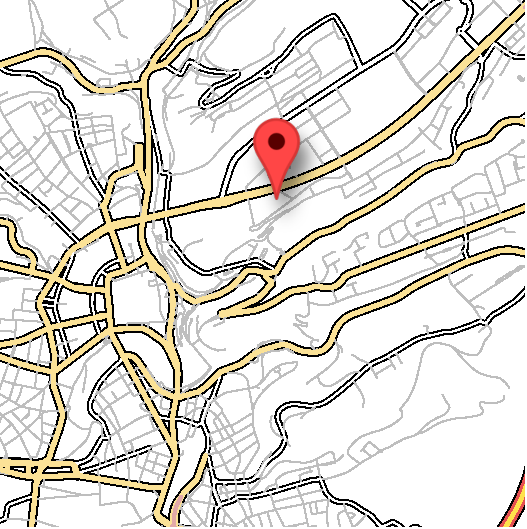
\includegraphics[width=\linewidth]{map.pdf}
        4 Place de l'Europe, 1499 Luxembourg
    }
    \end{tcolorbox}%
\end{minipage}%
\hspace{3cm}%
\begin{minipage}{7cm}
\begin{tcolorbox}[
    enhanced,
    width=7cm,
    before skip=2mm,after skip=2mm,
    colback=conference!5,colframe=conference!50,boxrule=0.2mm,
    attach boxed title to top left={xshift=1cm,yshift*=1mm-\tcboxedtitleheight},
    varwidth boxed title*=-2cm,
    boxed title style={frame code={
        \path[fill=tcbcolback!30!conference]
        ([yshift=-1mm,xshift=-1mm]frame.north west)
        arc[start angle=0,end angle=180,radius=1mm]
        ([yshift=-1mm,xshift=1mm]frame.north east)
        arc[start angle=180,end angle=0,radius=1mm];
        \path[left color=tcbcolback!60!conference,right color=tcbcolback!60!conference,
        middle color=tcbcolback!80!conference]
        ([xshift=-2mm]frame.north west) -- ([xshift=2mm]frame.north east)
        [rounded corners=1mm]-- ([xshift=1mm,yshift=-1mm]frame.north east)
        -- (frame.south east) -- (frame.south west)
        -- ([xshift=-1mm,yshift=-1mm]frame.north west)
        [sharp corners]-- cycle;
        },interior engine=empty,
    },
    fonttitle=\bfseries,
    title={Did you know}
]
    %\RaggedRight
    The First European Interstellar Symposium is part of the \textbf{Luxembourg Space Week} and is cohosted with 3 other parallel events in the same venue.
\end{tcolorbox}
\begin{tcolorbox}[
    enhanced,
    width=7cm,
    before skip=2mm,after skip=2mm,
    colback=MaterialGreen600!5,colframe=MaterialGreen600!50,boxrule=0.2mm,
    attach boxed title to top left={xshift=1cm,yshift*=1mm-\tcboxedtitleheight},
    varwidth boxed title*=-2cm,
    boxed title style={frame code={
        \path[fill=tcbcolback!30!MaterialGreen600]
        ([yshift=-1mm,xshift=-1mm]frame.north west)
        arc[start angle=0,end angle=180,radius=1mm]
        ([yshift=-1mm,xshift=1mm]frame.north east)
        arc[start angle=180,end angle=0,radius=1mm];
        \path[left color=tcbcolback!60!MaterialGreen600,right color=tcbcolback!60!MaterialGreen600,
        middle color=tcbcolback!80!MaterialGreen600]
        ([xshift=-2mm]frame.north west) -- ([xshift=2mm]frame.north east)
        [rounded corners=1mm]-- ([xshift=1mm,yshift=-1mm]frame.north east)
        -- (frame.south east) -- (frame.south west)
        -- ([xshift=-1mm,yshift=-1mm]frame.north west)
        [sharp corners]-- cycle;
        },interior engine=empty,
    },
    fonttitle=\bfseries,
    title={Stay updated}
]
    \RaggedRight
    \setlength{\parskip}{1ex}
    Follow the up-to-date version of the schedule online, at \url{https://feis2024.uni.lu/schedule}.

    This version was last updated\linebreak[4] on \today.
\end{tcolorbox}
\end{minipage}%
\end{center}

\newpage
\begin{center}
\color{white}\LARGE \centering \shadowtext{Keynote Events}
\end{center}


    \vfill
    \definecolor{thistrack}{HTML}{202020}

    \begin{tcolorbox}[
        enhanced,
        title={Keynote Lecture 1: Pete Worden (Breakthrough Initiatives) \\ Life in the Universe and Private Sector Space Science Initiatives},
        sharp corners,
        colbacktitle=thistrack,
        fonttitle=\large\mediumfont,
        boxsep=0pt,
        boxrule=0pt,
        left*=0pt,
        lefttitle=4mm,
        toptitle=4mm,
        bottomtitle=4mm,
        top=0pt,
        bottom=0pt,
        sidebyside,
        sidebyside align=center,
        lefthand width=6cm,
        segmentation empty,
    ]\begin{tikzpicture}[]%
            \draw node[outer sep=0,inner sep=0,anchor=north west] at (0,0) {%
                % wtf
                \adjincludegraphics[height=9.3cm,clip,trim={0 0 1cm 0}]{
                    media/keynote1.jpg}%
            };

            \fill[opacity=.7,black!50!thistrack] (0,-6.5) rectangle (current bounding box.south east);

            \draw node[white,anchor=south,yshift=5mm] (DAY) at (current bounding box.south) {
                \timeregularfont\Huge \scalebox{.8}[1.0]{%
                    TUESDAY%
                }%
            };

            \draw node[white,above of=DAY] (TIME)  {
                \timeregularfont\Large 09:00 \textendash~ 09:50 
            };
        \end{tikzpicture}%
        
        \tcblower

        \setlength{\parskip}{1ex}
        
        \vspace{1ex}
        Dr.~Worden will present Breakthrough Listen, looking for signs of extraterrestrial technology; Breakthrough Watch, looking for nearby exoplanets; Breakthrough Starshot, engineering a light-driven probe for Alpha Centauri; and other space science programs to find life beyond earth and explore the cosmos.

        {
            \small
            \color{white!20!black}
            Dr.~S.~``Pete''' Worden, (Brig Gen, USAF, Ret, PhD) is Chairman of the Breakthrough Prize Foundation and Executive Director of the foundation's ``Breakthrough Initiatives''. He holds a Bachelor of Science degree in Physics and Astronomy from the University of Michigan and a PhD in Astronomy from the University of Arizona. After several US Air Force positions and a research professorship in astronomy at the University of Arizona, Dr.~Worden was Director of NASA's Ames Research Center until retiring on March 31, 2015. From 2017 to the present, Brigadier General Worden is an Advisor to the Luxembourg Space Agency and was appointed as a Knight-Commander of the Order of Merit of the Grand Duchy of Luxembourg in 2018 for his space services.}

        

        \vspace{2ex}
    \end{tcolorbox}
    \vspace{-1ex}

    \vfill
    \definecolor{thistrack}{HTML}{202020}

    \begin{tcolorbox}[
        enhanced,
        title={Keynote Lecture 2: Slava Turyshev (NASA Jet Propulsion Laboratory) \\  Multipixel Imaging and Spectroscopy of Exoplanets — A Search for Life with the Solar Gravitational Lens},
        sharp corners,
        colbacktitle=thistrack,
        fonttitle=\large\mediumfont,
        boxsep=0pt,
        boxrule=0pt,
        left*=0pt,
        lefttitle=4mm,
        toptitle=4mm,
        bottomtitle=4mm,
        top=0pt,
        bottom=0pt,
        sidebyside,
        sidebyside align=center,
        lefthand width=6cm,
        segmentation empty,
    ]\begin{tikzpicture}[]%
            \draw node[outer sep=0,inner sep=0,anchor=north west] at (0,0) {%
                % wtf
                \adjincludegraphics[height=9.3cm,clip,trim={1.5cm 0 0.5cm 0}]{
                    media/keynote6.jpg}%
            };

            \fill[opacity=.7,black!50!thistrack] (0,-6.5) rectangle (current bounding box.south east);

            \draw node[white,anchor=south,yshift=5mm] (DAY) at (current bounding box.south) {
                \timeregularfont\Huge \scalebox{.8}[1.0]{%
                    TUESDAY%
                }%
            };

            \draw node[white,above of=DAY] (TIME)  {
                \timeregularfont\Large 13:30 \textendash~ 14:20 
            };
        \end{tikzpicture}%
        
        \tcblower

        \setlength{\parskip}{1ex}
        
        \vspace{1ex}
        The Solar Gravitational Lens (SGL) is a natural phenomenon caused by the Sun's gravitational field bending and focusing light, as predicted by general relativity. This effect provides extraordinary light amplification and angular resolution, enabling detailed imaging and spectroscopy of faint targets. A modest telescope positioned in SGL's focal region, beginning at $\sim$548 AU, could exploit it to achieve high-resolution imaging of exoplanets. This presentation discusses SGL's properties and introduces a mission concept enabled by solar sail propulsion. Sailcraft technologies are expected to allow heliocentric velocities of 20–25 AU/year within 5–7 years, enabling practical missions within two decades.

        {
            \small
            \color{white!20!black}
            Slava G.\ Turyshev is an astrophysicist at NASA's JPL, Caltech, and a professor in the Department of Physics and Astronomy at UCLA. His research focuses on gravitational and fundamental physics, relativistic astrophysics, gravitational waves, and planetary science. He served as the NASA Project Scientist for the CNES/ESA MICROSCOPE mission, as the Principal Investigator for the Advanced Lunar Laser Ranging Facility, the Pioneer Anomaly investigation, and NASA Innovative Advanced Concepts (NIAC) Phases I–III, and as a member of the Executive Committee of NASA’s Fundamental Physics Advisory Group (FunPAG).}

        

        \vspace{2ex}
    \end{tcolorbox}
    \vspace{-1ex}

    \vfill
    \definecolor{thistrack}{HTML}{202020}

    \begin{tcolorbox}[
        enhanced,
        title={Keynote Lecture 3: Richard A.\ Norte (Delft University of Technology) \\ Propelling Interstellar Exploration: Extreme-Aspect-Ratio Metamaterials in a Post-Moore Era},
        sharp corners,
        colbacktitle=thistrack,
        fonttitle=\large\mediumfont,
        boxsep=0pt,
        boxrule=0pt,
        left*=0pt,
        lefttitle=4mm,
        toptitle=4mm,
        bottomtitle=4mm,
        top=0pt,
        bottom=0pt,
        sidebyside,
        sidebyside align=center,
        lefthand width=6cm,
        segmentation empty,
    ]\begin{tikzpicture}[]%
            \draw node[outer sep=0,inner sep=0,anchor=north west] at (0,0) {%
                % wtf
                \adjincludegraphics[height=9.3cm,clip,trim={1.9cm 0 1.4cm 0}]{
                    media/keynote7.jpg}%
            };

            \fill[opacity=.7,black!50!thistrack] (0,-6.5) rectangle (current bounding box.south east);

            \draw node[white,anchor=south,yshift=5mm] (DAY) at (current bounding box.south) {
                \timeregularfont\Huge \scalebox{.8}[1.0]{%
                    TUESDAY%
                }%
            };

            \draw node[white,above of=DAY] (TIME)  {
                \timeregularfont\Large 15:50 \textendash~ 16:40 
            };
        \end{tikzpicture}%
        
        \tcblower

        \setlength{\parskip}{1ex}
        
        \vspace{1ex}
        For the past half century, Moore's Law has steered the course of nanotechnology, propelling miniaturization in all 3 dimensions. As we approach its limits, our lab is exploring a new kind of nanotechnology that extends to large distances in the $X$ and $Y$ axes while remaining nanoscale in $Z$. The unique properties of these extreme-aspect-ratio metamaterials can advance applications such as missions that aim to reach Alpha Centauri in 20 years, instead of the 10\,000 years possible today. This talk will examine opportunities arising from the integration of advanced nanofabrication and high-power optomechanical experiments, as well as our efforts to use lightsail materails to stably levitate objects over 100\,000 times more massive than anything levitated with laser light to date.

        {
            \small
            \color{white!20!black}
            Richard A.\ Norte is a faculty member at TU Delft in the Netherlands. His research group develops cutting-edge nanotechnologies for quantum hardware. His work has been featured in Nature, Nature Photonics, Science, Physical Review Letters, and on the cover of Scientific American. His team has achieved significant breakthroughs in laser sail nano-manufacturing, reducing fabrication times from 15 years to a single day by integrating nanophotonics, fabrication techniques, and economic considerations of the Starshot mission.}

        

        \vspace{2ex}
    \end{tcolorbox}
    \vspace{-1ex}

    \vfill
    \definecolor{thistrack}{HTML}{5FAB5D}

    \begin{tcolorbox}[
        enhanced,
        title={Public Outreach Event: Sara Seager (MIT) \\ An Enduring Mystery of Astronomy: Can We Find Signs of Life Beyond Earth?},
        sharp corners,
        colbacktitle=thistrack,
        fonttitle=\large\mediumfont,
        boxsep=0pt,
        boxrule=0pt,
        left*=0pt,
        lefttitle=4mm,
        toptitle=4mm,
        bottomtitle=4mm,
        top=0pt,
        bottom=0pt,
        sidebyside,
        sidebyside align=center,
        lefthand width=6cm,
        segmentation empty,
    ]\begin{tikzpicture}[]%
            \draw node[outer sep=0,inner sep=0,anchor=north west] at (0,0) {%
                % wtf
                \adjincludegraphics[height=9.3cm,clip,trim={3.4cm 0 5.6cm 0}]{
                    media/public2.jpg}%
            };

            \fill[opacity=.7,black!50!thistrack] (0,-6.5) rectangle (current bounding box.south east);

            \draw node[white,anchor=south,yshift=5mm] (DAY) at (current bounding box.south) {
                \timeregularfont\Huge \scalebox{.8}[1.0]{%
                    TUESDAY%
                }%
            };

            \draw node[white,above of=DAY] (TIME)  {
                \timeregularfont\Large 18:30 \textendash~ 20:00 
            };
        \end{tikzpicture}%
        
        \tcblower

        \setlength{\parskip}{1ex}
        
        \vspace{1ex}
        For thousands of years, people have wondered what lies beyond Earth. Today, astronomers have discovered thousands of exoplanets, and JWST is studying gases in exoplanet atmospheres, including those that might indicate life. Renewed interest in Venus has sparked investigations into the potential for life there, fueled by controversial phosphine detections and laboratory studies of organic molecules' stability in Venus's sulfuric acid clouds. Prof.~Seager will share the latest advances in this exciting field.

        {
            \small
            \color{white!20!black}
            Prof.~Sara Seager, a Canadian-American astrophysicist and planetary scientist, finds inspiration in the vastness of space. Currently the Class of 1941 Professor of Planetary Science, Professor of Physics, and Professor of Aeronautical and Astronautical Engineering at the Massachusetts Institute of Technology, she pioneered numerous techniques for characterizing exoplanets, revolutionizing our ability to understand these distant worlds. Seager has garnered global recognition, including a MacArthur Fellowship, the 2024 Kavli Prize in Astrophysics, appointment as an Officer of the Order of Canada, and has asteroid 9729 named in her honor.}

        
        \begin{tcolorbox}[
            % round corners,
            frame hidden,
            sidebyside,
            bicolor,
            colback=thistrack!70!black,
            colbacklower=thistrack!90!black,
            %#sharp corners=downhill,
            size=title,
            boxrule=0pt,
            lefthand ratio=0.6,
            sidebyside align=center,
            halign=center,
            halign lower=flush center,
            % title={  },
        ]%
            \color{white}%
            \textbf{%
                FREE REGISTRATION REQUIRED%
            }%
            \tcblower%
            \color{white}%
            \footnotesize\url{https://feis2024.uni.lu/register/seager}%
        \end{tcolorbox}
        

        \vspace{2ex}
    \end{tcolorbox}
    \vspace{-1ex}

    \vfill
    \definecolor{thistrack}{HTML}{202020}

    \begin{tcolorbox}[
        enhanced,
        title={Keynote Lecture 4: Paolo Villoresi (University of Padova) \\  Harnessing the light emission for extreme space optical communication},
        sharp corners,
        colbacktitle=thistrack,
        fonttitle=\large\mediumfont,
        boxsep=0pt,
        boxrule=0pt,
        left*=0pt,
        lefttitle=4mm,
        toptitle=4mm,
        bottomtitle=4mm,
        top=0pt,
        bottom=0pt,
        sidebyside,
        sidebyside align=center,
        lefthand width=6cm,
        segmentation empty,
    ]\begin{tikzpicture}[]%
            \draw node[outer sep=0,inner sep=0,anchor=north west] at (0,0) {%
                % wtf
                \adjincludegraphics[height=9.3cm,clip,trim={0 0 0 0}]{
                    media/keynote3.png}%
            };

            \fill[opacity=.7,black!50!thistrack] (0,-6.5) rectangle (current bounding box.south east);

            \draw node[white,anchor=south,yshift=5mm] (DAY) at (current bounding box.south) {
                \timeregularfont\Huge \scalebox{.8}[1.0]{%
                    WEDNESDAY%
                }%
            };

            \draw node[white,above of=DAY] (TIME)  {
                \timeregularfont\Large 09:00 \textendash~ 09:50 
            };
        \end{tikzpicture}%
        
        \tcblower

        \setlength{\parskip}{1ex}
        
        \vspace{1ex}
        We present the study of the communication system designed to transmit data from an ultralight sail on an interplanetary mission. By estimating parameters such as divergence and power required, we arrive at the dimensioning of the transmitter, achieved with phased-array grating couplers. Some implementation models and the optimal error-correction code for these devices are presented. By drawing inspiration from Quantum Communication in space, the preparation of the pulses can also provide significant metrological information for studying the kinematics of solar sails.

        {
            \small
            \color{white!20!black}
            Paolo Villoresi is a Professor of Physics and Director of the Padua Quantum Technologies Research Center at the University of Padova. He realized the first single photon exchange with a satellite and demonstrated the first Quantum Communication in space using orbiting retroreflectors. His past research topics include Atomic Physics in the attosecond domain, the generation of high-order harmonics, multiphoton ionization, and ultrafast optics in extreme UV and X-ray domains. He has deposited 14 industrial patents and patent applications. He is the President of the Strategic Technical Committee of Veneto Sviluppo and founder of ThinkQuantum, a spinoff of University of Padova introducing advanced QKD technologies for space and ground networks.}

        

        \vspace{2ex}
    \end{tcolorbox}
    \vspace{-1ex}

    \vfill
    \definecolor{thistrack}{HTML}{202020}

    \begin{tcolorbox}[
        enhanced,
        title={Keynote Lecture 5: Martin Tajmar (TU Dresden) \\  Overview of Breakthrough Propulsion at TU Dresden},
        sharp corners,
        colbacktitle=thistrack,
        fonttitle=\large\mediumfont,
        boxsep=0pt,
        boxrule=0pt,
        left*=0pt,
        lefttitle=4mm,
        toptitle=4mm,
        bottomtitle=4mm,
        top=0pt,
        bottom=0pt,
        sidebyside,
        sidebyside align=center,
        lefthand width=6cm,
        segmentation empty,
    ]\begin{tikzpicture}[]%
            \draw node[outer sep=0,inner sep=0,anchor=north west] at (0,0) {%
                % wtf
                \adjincludegraphics[height=9.3cm,clip,trim={2.5cm 0 2cm 0}]{
                    media/keynote4.jpg}%
            };

            \fill[opacity=.7,black!50!thistrack] (0,-6.5) rectangle (current bounding box.south east);

            \draw node[white,anchor=south,yshift=5mm] (DAY) at (current bounding box.south) {
                \timeregularfont\Huge \scalebox{.8}[1.0]{%
                    WEDNESDAY%
                }%
            };

            \draw node[white,above of=DAY] (TIME)  {
                \timeregularfont\Large 13:30 \textendash~ 14:20 
            };
        \end{tikzpicture}%
        
        \tcblower

        \setlength{\parskip}{1ex}
        
        \vspace{1ex}
        Human exploration to the stars will require a breakthrough in propulsion. We therefore decided to establish a dedicated breakthrough propulsion group within our institute to investigate and test new ideas for propellantless propulsion. Our main focus is developing a cutting-edge suite of measurement devices including thrust balances with (sub) nano-Newton resolution and a superconducting levitation thrust stand as well as a nano-gram weight balance. Several tests were carried out to test claims of revolutionary propulsion devices such as the EMDrive that could be traced back to setup-related artefacts. Here we review our program goals and developments and show some examples of what we tested so far as well as what we want to do in the future.

        {
            \small
            \color{white!20!black}
            Prof.~Dr.~Martin Tajmar studied physics, space studies and electrical engineering, graduating with a PhD from TU Wien. After research stays at NASA JPL and ESA-ESTEC, he joined the Austrian Institute of Technology where he was head of the business unit ``Space Propulsion \& Advanced Concepts''. After being appointed as associate professor at KAIST, he moved to TU Dresden as full professor and head of the chair of space systems in 2012, where he later became the director of the Institute of Aerospace Engineering.}

        

        \vspace{2ex}
    \end{tcolorbox}
    \vspace{-1ex}

    \vfill
    \definecolor{thistrack}{HTML}{202020}

    \begin{tcolorbox}[
        enhanced,
        title={Keynote Lecture 6: Harry Atwater (California Institute of Technology) \\  StarShot \textemdash~from physics to spacecraft},
        sharp corners,
        colbacktitle=thistrack,
        fonttitle=\large\mediumfont,
        boxsep=0pt,
        boxrule=0pt,
        left*=0pt,
        lefttitle=4mm,
        toptitle=4mm,
        bottomtitle=4mm,
        top=0pt,
        bottom=0pt,
        sidebyside,
        sidebyside align=center,
        lefthand width=6cm,
        segmentation empty,
    ]\begin{tikzpicture}[]%
            \draw node[outer sep=0,inner sep=0,anchor=north west] at (0,0) {%
                % wtf
                \adjincludegraphics[height=9.3cm,clip,trim={0.3cm 0 1cm 0}]{
                    media/keynote2.jpg}%
            };

            \fill[opacity=.7,black!50!thistrack] (0,-6.5) rectangle (current bounding box.south east);

            \draw node[white,anchor=south,yshift=5mm] (DAY) at (current bounding box.south) {
                \timeregularfont\Huge \scalebox{.8}[1.0]{%
                    WEDNESDAY%
                }%
            };

            \draw node[white,above of=DAY] (TIME)  {
                \timeregularfont\Large 15:50 \textendash~ 16:40 
            };
        \end{tikzpicture}%
        
        \tcblower

        \setlength{\parskip}{1ex}
        
        \vspace{1ex}
        Over the last several years, significant progress has been made on the understanding of the requirements for design of laser-driven lightsails suitable for interstellar missions. Nanophotonic design principles can enable self-stabilizing optical manipulation, levitation and propulsion of ultralight microscopic and macroscopic-sized (i.e., micron, mm, cm, or even meter-scale) metasurface lightsails via radiation pressure from a high power density pump laser source. I will discuss new simulations and measurements to test the stringent criteria for metasurface lightsail design, dynamical and opto-mechanical stability, and thermal management.

        {
            \small
            \color{white!20!black}
            Harry Atwater is the Otis Booth Leadership Chair of the Division of Engineering and Applied Science, and the Howard Hughes Professor of Applied Physics and Materials Science at the California Institute of Technology. Atwater's scientific effort focuses on nanophotonic light-matter interactions. He was an early pioneer in nanophotonics and plasmonics and gave a name to the field of plasmonics in 2001. Atwater's work spans fundamental nanophotonic phenomena and applications, including active wavefront shaping of light using metasurfaces, optical propulsion of lightsails, quantum and 2D nanophotonics as well as solar energy conversion, on earth and in space.}

        

        \vspace{2ex}
    \end{tcolorbox}
    \vspace{-1ex}

    \vfill
    \definecolor{thistrack}{HTML}{202020}

    \begin{tcolorbox}[
        enhanced,
        title={Keynote Lecture 7: Mona Nasser (University of Plymouth) \\  Voyaging Through the Vast \textemdash~Transforming Clinical Research Methods for Interstellar Expeditions},
        sharp corners,
        colbacktitle=thistrack,
        fonttitle=\large\mediumfont,
        boxsep=0pt,
        boxrule=0pt,
        left*=0pt,
        lefttitle=4mm,
        toptitle=4mm,
        bottomtitle=4mm,
        top=0pt,
        bottom=0pt,
        sidebyside,
        sidebyside align=center,
        lefthand width=6cm,
        segmentation empty,
    ]\begin{tikzpicture}[]%
            \draw node[outer sep=0,inner sep=0,anchor=north west] at (0,0) {%
                % wtf
                \adjincludegraphics[height=9.3cm,clip,trim={3.9cm 0 3.9cm 0}]{
                    media/keynote5.jpg}%
            };

            \fill[opacity=.7,black!50!thistrack] (0,-6.5) rectangle (current bounding box.south east);

            \draw node[white,anchor=south,yshift=5mm] (DAY) at (current bounding box.south) {
                \timeregularfont\Huge \scalebox{.8}[1.0]{%
                    THURSDAY%
                }%
            };

            \draw node[white,above of=DAY] (TIME)  {
                \timeregularfont\Large 09:00 \textendash~ 09:50 
            };
        \end{tikzpicture}%
        
        \tcblower

        \setlength{\parskip}{1ex}
        
        \vspace{1ex}
        Human adaptation to the ever-changing conditions of interstellar travel presents unprecedented challenges to our understanding of health and medicine. Despite our efforts, unexpected challenges are inevitable during long-duration interstellar missions. This raises a crucial question: How can we adapt clinical research to develop a more responsive and resilient healthcare infrastructure for interstellar ventures? This presentation will explore innovative methodological approaches that could enhance our preparedness for interstellar travel, based on insights from a series of MetaFuturism Lab workshops.

        {
            \small
            \color{white!20!black}
            Mona Nasser is the Director of the Plymouth Institute of Health and Care Research (PIHR) and a Professor of Clinical Epidemiology and Oral Health Research at the University of Plymouth. She is a methodologist, health services researcher, and interdisciplinary scientist. She has been working with members of the Space Medicine Team at the European Astronaut Centre on the Systematic Threat Analysis of Radiation from Space (STARS) project and leads a research group on the Impact of Space Environment on Craniofacial and Dental Structure (ISECS) at the university.}

        

        \vspace{2ex}
    \end{tcolorbox}
    \vspace{-1ex}


% Sponsor Logos

\vfill

\begin{tcolorbox}[
    width=\paperwidth,center,boxrule=0pt,arc=0pt,auto outer arc,colframe=white,colback=white,valign=center]
    %
    \hfill
    \raisebox{-0.5\height}{
\includegraphics[width=2.5cm]{media/logo1.jpeg}}
    \hfill
    \raisebox{-0.5\height}{
\includegraphics[width=3cm]{media/logo3.png}}
    \hfill
    \raisebox{-0.5\height}{
\includegraphics[width=2cm]{media/logo4.png}}
    \hfill
    \raisebox{-0.5\height}{
\includegraphics[width=1.9cm]{media/logo7.png}}
    \hfill
    \raisebox{-0.5\height}{\adjincludegraphics[width=3.7cm,trim={1.5cm 0 3.5cm 0},clip]{media/logo5.png}}
    \hfill
    \raisebox{-0.5\height}{
\includegraphics[width=3.5cm]{media/logo8.png}}
    \hfill
\end{tcolorbox}

\begin{center}%
\color{white!80!black}%
Background designed by Maciej Rebisz for Science Now
\end{center}

\vspace{1cm}

\end{document}